\section{レンズと球面鏡}

% ===========================================================================
%  再編（2026-09-10）：第2章 波動 の第20回（波動の最終回）．
%  原本の 第27回「レンズ(1)」（27.1 凸レンズ／27.2 凹レンズ／27.3 虚光源／
%  27.4 凹面鏡・凸面鏡）と 第28回「レンズ(2)」（28.1 写像公式／28.2 偏光）を
%  1回にまとめた（前半＝作図，後半＝写像公式）。
%  ・例題は原本【例題26】〜【例題31】の6題をそのまま採用した（削除なし）。
%    例題26＝原本㉗[60]，例題27＝㉗[61]，例題30＝㉘[68] と**問題が完全に同一**なので，
%    練習側では A問題4題（㉗[60][61]・㉘[68][69]）を1題に統合し，
%    実質 ㉘[69]〈光の現象〉だけを残した（再編案の「A4→1」はこの統合を指す）。
%    設問は1つも失われていない（[60][61][68] の設問は例題26・27・30 に全部ある）。
%  ・練習は ㉗[62]〜[67] ＋ ㉘[70]〜[75] ＋ 統合したA問題 の13題（［63］〜［75］）。
%    ㉘章末[76]は第19回で削除，㉘章末[77]は第19回の［62］へ移してある。
%  ・原本の誤植を4件直した（すべてコメントで明記）。
% ===========================================================================

% 例題番号：波動（原本 第3章）の例題は章の先頭から1・2・3…と振られており，再編でも
% 例題の順序は変わらないので，原本の番号がそのまま使える（第20回は【例題26】から）。
%   新14 ＝ 原本例題1〜5／新15 ＝ 6〜9／新16 ＝ 10〜12／新17 ＝ 13〜19／
%   新18 ＝ 20〜22／新19 ＝ 23〜25／新20 ＝ 26〜31
\setcounter{nombre}{25}

\subsection{凸レンズ}

\begin{zuright}{70mm}
\hspace{1zw}レンズは光の屈折を利用して光を集めたり発散させたりすることができるもので，2つの球面によって挟まれたガラスなどで出来ている．レンズには凸レンズと凹レンズがあるが，まず凸レンズについて考えてみよう．

\hspace{1zw}レンズの2つの球面の中心を結ぶ直線をレンズの{\gtfamily 光軸}という．光軸に対して平行な光線を凸レンズにあてると，光はレンズの後方（向こう側）のある一点$\mathrm{F}$に集まる．この点$\mathrm{F}$をそのレンズの{\gtfamily 焦点}といい，レンズの中心から焦点までの距離をレンズの{\gtfamily 焦点距離}という．

% 加筆（2026-09-10）：レンズの理論が「薄いレンズ・近軸近似」の上に成り立っていることが
% 本文のどこにも書かれておらず，20.1 の「（レンズの厚さが無視できるとき）」という括弧書きだけが
% 暗黙の前提になっていた。例題・練習には「近軸近似」という語のタイトルが付いた問題がある。
% zuright の「中」に置くこと：左の本文(7行)は図(82.6mm＝14.8行)より短いので，ここに
% 数行足してもページの高さは変わらない。外に出すと講義部が1ページ増える（実測済み）。
\hspace{1zw}以下で述べるレンズの性質と 20.5 の写像公式は，いずれも{\gtfamily レンズの厚さが無視できるほど薄く（薄いレンズ），光線が光軸の近くを通る}という条件（{\gtfamily 近軸近似}）のもとで成り立つ．以下では特に断らない限りこの条件が成り立つものとする．
\zusep

\includegraphics[keepaspectratio,width=70mm]{text2_p15_fig1.png}
\end{zuright}

\hspace{1zw}レンズの焦点はレンズの前方と後方にひとつずつあり，いずれの焦点距離も等しい．焦点に光源を置いた場合は先ほどのちょうど逆向きとなり，レンズを通ると光軸に平行な光線群となる．

\hspace{1zw}次に，レンズより小さいサイズの物体を光軸上，手前の焦点よりも外側に置き，物体のある点$\mathrm{P}$から出ていく以下の3つの光について考える．

\begin{zuright}{88mm}
\hspace{1zw}\MARU{1}\hspace{2mm}{\gtfamily 光軸に平行に出た光}

\hspace{2zw}この光はレンズの向こう側の焦点を通るように進む．

\hspace{1zw}\MARU{2}\hspace{2mm}{\gtfamily レンズの中心を通過する光}

\hspace{2zw}この光は曲がらずに直進する．（レンズの厚さが無視できるとき）

\hspace{1zw}\MARU{3}\hspace{2mm}{\gtfamily 手前側の焦点を通る光}

\hspace{2zw}この光はレンズの向こう側に出ると光軸に平行な光線となる．
\zusep

\includegraphics[keepaspectratio,width=88mm]{text2_p15_fig2.png}
\end{zuright}

\hspace{1zw}今は3つのみについて考えたが，点$\mathrm{P}$から出てレンズに入った光は\MARU{1}, \MARU{2}, \MARU{3}に限らず，{\gtfamily すべて同一の点$\mathrm{Q}$を通る．}そのため，光軸に対して垂直で$\mathrm{Q}$点を含む面に紙を置くと，紙面には光源の像が生じる．この像のように，実際に光が集まって作られる像を{\gtfamily 実像}と呼ぶ．この場合，像は光源の物体に対して逆さまになっているので，これを{\gtfamily 倒立像}と呼ぶ．これに対し像が同じ向きになっているものは{\gtfamily 正立像}と呼ぶ．

\hspace{1zw}なお，実際の像の位置の把握には，上述の3つのうち2つを考えれば十分である．

%%%%% 例題26（27.1 の直後）＝ 原本【例題26】〈凸レンズの像の作図〉 %%%%%%%%%%%%%
% 問題文・【KEY】は原本（p16）からの転写。原本には解答が載っていないので解答は書き起こした。
% 図は㉗[60]と同一なので問題編スキャン prob2_p11 から切り出した。
% 解答の図は㉗[60]の解答（prob2_p83_2）から切り出したものをそのまま使える。
\bsNeed{62mm}
\begin{reidaiunit}
\begin{reidai}{凸レンズの像の作図}
\begin{zuright}{76mm}
\hspace{1zw}焦点が$\mathrm{F_1}$, $\mathrm{F_2}$であるような凸レンズがある．レンズに対して図のような位置に物体$\mathrm{AA^\prime}$を置き，この像を観察する．
\begin{komon}
\ko{1} 物体$\mathrm{AA^\prime}$の像$\mathrm{BB^\prime}$を作図せよ．
\ko{2} $\mathrm{A}$点から図のように凸レンズに入射した光の屈折光を作図せよ．
\end{komon}
\zusep
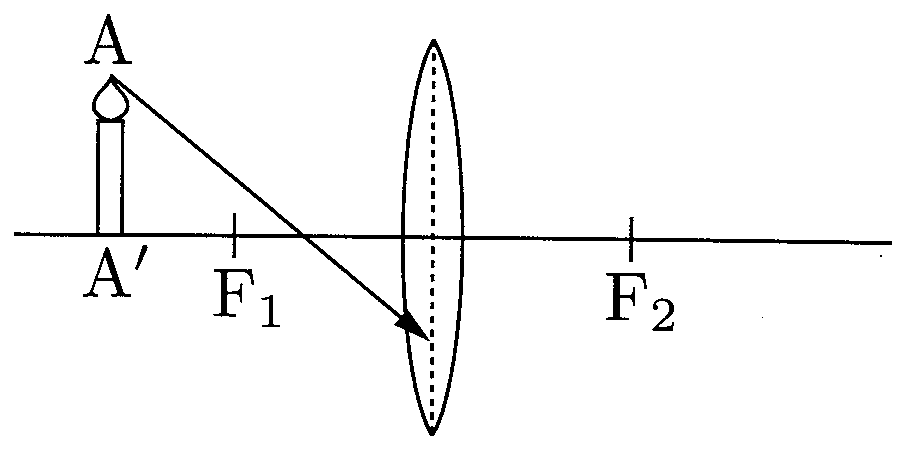
\includegraphics[keepaspectratio,width=76mm]{fig/n20_ex26.png}
\end{zuright}
\end{reidai}

\begin{sisinE}
レンズによる屈折光を作図するには，{\gtfamily \MARU{1}光軸に平行に出て向こう側の焦点を通るような光}，{\gtfamily \MARU{2}レンズの中心$\mathrm{O}$を通過してそのまま直進する光}，の二つを作図し，交点を求めよ．レンズに入射する光はすべてその交点を通るので，(2)ではレンズに入った光がその交点に向かうと考えて作図すればよい．
\end{sisinE}

\Key{\MARU{1} 光軸に平行に出た光　\MARU{2} レンズの中心を通過する光　\MARU{3} 手前側の焦点を通る光\\
\hspace*{1zw}のうち，2つの光線の交点を作図する．}

\begin{kaitou}
\begin{komon}
\ko{1} $\mathrm{A}$点から出て，\MARU{1}光軸に平行に出て向こう側の焦点を通るような光，\MARU{2}レンズの中心$\mathrm{O}$を通過してそのまま直進する光，の二つを作図して交点を得ると図の$\mathrm{B}$点となるので，この位置に像が出来る．よって，凸レンズにより出来る像は図の$\mathrm{BB^\prime}$（\AnaU{\gtfamily 倒立実像}）となる．
       \begin{center}\AnaFig{76mm}{fig/n20_ex26_ans1.png}{fig/n20_ex26_blank1.png}\end{center}
\ko{2} $\mathrm{A}$点から凸レンズに入射した光はすべて図の$\mathrm{B}$点に収束するので，$\mathrm{B}$点に向かうような方向へ屈折する．よってレンズによる屈折光は次図のようになる．
       \begin{center}\AnaFig{76mm}{fig/n20_ex26_ans2.png}{fig/n20_ex26_blank2.png}\end{center}
\end{komon}
\end{kaitou}
\end{reidaiunit}

\subsection{凹レンズ}

\begin{zuright}{70mm}
\hspace{1zw}凹レンズは周辺部よりも中心部の方がへこんでいる形のレンズである．凹レンズの光軸に対して平行な光線をあてると，光はレンズを通ると図のように広がっていく．この広がっていく光線をレンズの手前側まで伸ばすと，直線はある一点で交わる．すなわち，レンズにより発散した光線はこの一点から直進して出ていった光と同様になる．この点を凹レンズの{\gtfamily 焦点}という．

\hspace{1zw}凹レンズについても凸レンズ同様，レンズの前方と後方に焦点がひとつずつあり，その焦点距離はいずれも等しい．またレンズの向こう側にある焦点に光を集めるように凹レンズに光を入射すると，その光は凹レンズを通過した後，光軸に平行な光線群となる．
\zusep

\includegraphics[keepaspectratio,width=70mm]{text2_p16_fig1.png}
\end{zuright}

\hspace{1zw}次にレンズより小さいサイズの物体を光軸上，焦点よりも外側に置き，物体のある点$\mathrm{P}$から出ていく以下の3つの光について考える．

\begin{zuright}{88mm}
\hspace{1zw}\MARU{1}\hspace{2mm}{\gtfamily 光軸に平行に出た光}

\hspace{2zw}この光はレンズの手前側の焦点から直進するように進む．

\hspace{1zw}\MARU{2}\hspace{2mm}{\gtfamily レンズの中心を通過する光}

\hspace{2zw}この光は曲がらずに直進する．（レンズの厚さが無視できるとき）

\hspace{1zw}\MARU{3}\hspace{2mm}{\gtfamily 向こう側の焦点へ直進する光}

\hspace{2zw}この光はレンズの向こう側に出ると光軸に平行な光線となる．
\zusep

\includegraphics[keepaspectratio,width=88mm]{text2_p17_fig1.png}
\end{zuright}

\hspace{1zw}レンズの向こう側に出た\MARU{1}〜\MARU{3}の3つの光線はレンズの向こう側では交わらないが，これらの光線をレンズの手前側に戻してやると，それらは図の$\mathrm{Q}$点の一点に交わる．すなわち，レンズの向こう側の光線は，$\mathrm{Q}$の位置から直進して出てきた光のように広がっていく．そのため，レンズの向こう側からレンズを覗き見るとあたかも$\mathrm{Q}$に物体があるかのように見える．この$\mathrm{Q}$を{\gtfamily 虚像}という．虚像は実像と異なり，実際にその位置に光が集まってはいないため虚像の位置に紙を置いても像は写らない．

%%%%% 例題27 ＝ 原本【例題27】〈凹レンズの像の作図〉 %%%%%%%%%%%%%%%%%%%%%%%%%%%
\bsNeed{62mm}
\begin{reidaiunit}
\begin{reidai}{凹レンズの像の作図}
\begin{zuright}{76mm}
\hspace{1zw}焦点が$\mathrm{F_1}$, $\mathrm{F_2}$であるような凹レンズがある．レンズに対して図のような位置に物体$\mathrm{AA^\prime}$を置き，この像を観察する．
\begin{komon}
\ko{1} 物体$\mathrm{AA^\prime}$の像$\mathrm{BB^\prime}$を作図せよ．
\ko{2} $\mathrm{A}$点から図のように凹レンズに入射した光の屈折光を作図せよ．
\end{komon}
\zusep
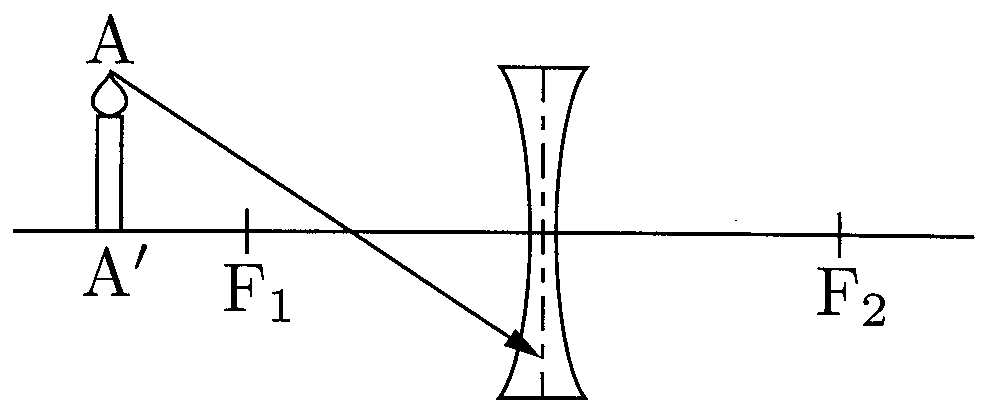
\includegraphics[keepaspectratio,width=76mm]{fig/n20_ex27.png}
\end{zuright}
\end{reidai}

\begin{sisinE}
凹レンズによる屈折光の作図も，{\gtfamily \MARU{1}光軸に平行に出て手前側の焦点から直進したかのように進む光}，{\gtfamily \MARU{2}レンズの中心$\mathrm{O}$を通過してそのまま直進する光}，の二つを作図して考える．この\MARU{1}, \MARU{2}の二つの光の交点がない場合にはレンズの手前側まで二つの線を延ばして交点を取り，この点に虚像が出来ると考えよ．レンズに入射する光はすべてこの交点から直進したかのように進むので，(2)ではレンズに入った光が交点からレンズを通って直進したと考えて作図すればよい．
\end{sisinE}

\Key{\MARU{1} 光軸に平行に出た光　\MARU{2} レンズの中心を通過する光　\MARU{3} 向こう側の焦点へ直進する光\\
\hspace*{1zw}のうち，2つの光線の交点を作図する．}

\begin{kaitou}
\begin{komon}
\ko{1} $\mathrm{A}$点から出て，\MARU{1}光軸に平行に出て手前側の焦点から直進したかのように進む光，\MARU{2}レンズの中心$\mathrm{O}$を通過してそのまま直進する光，の二つを作図するとこれらは交点を持たない．\MARU{1}をレンズの手前側まで延ばして交点を得ると図の$\mathrm{B}$点となるので，この位置に像が出来る．よって，凹レンズにより出来る像は図の$\mathrm{BB^\prime}$（\AnaU{\gtfamily 正立虚像}）となる．
       \begin{center}\AnaFig{76mm}{fig/n20_ex27_ans1.png}{fig/n20_ex27_blank1.png}\end{center}
\ko{2} $\mathrm{A}$点から凹レンズに入射した光はすべて図の$\mathrm{B}$点から出てレンズを直進したかのように進むので，$\mathrm{B}$点に向かうような方向へ屈折する．よってレンズによる屈折光は次図のようになる．
       \begin{center}\AnaFig{76mm}{fig/n20_ex27_ans2.png}{fig/n20_ex27_blank2.png}\end{center}
\end{komon}
\end{kaitou}
\end{reidaiunit}

%%%%% 例題28 ＝ 原本【例題28】〈レンズによる像の作図〉 %%%%%%%%%%%%%%%%%%%%%%%%%
% 原本に解答図が無いので，解答図は TikZ で自作した（texify_draft/mkfig_new20ans.py）。
\bsNeed{76mm}
\begin{reidaiunit}
\begin{reidai}{レンズによる像の作図}
\hspace{1zw}焦点が$\mathrm{F_1}$, $\mathrm{F_2}$であるような凸レンズ，凹レンズがある．レンズに対して図のような位置に物体$\mathrm{AA^\prime}$を置き，この像を観察するとき，各図について物体$\mathrm{AA^\prime}$の像$\mathrm{BB^\prime}$を作図し，像の種類を述べよ．
\begin{center}
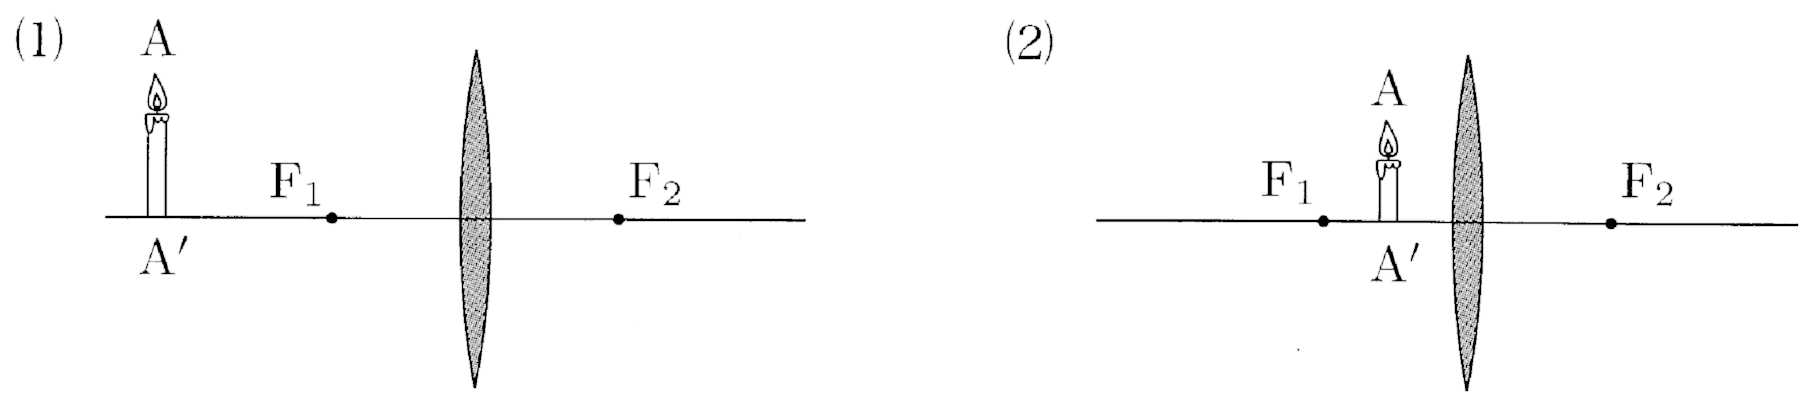
\includegraphics[keepaspectratio,width=128mm]{fig/n20_ex28a.png}\\[2mm]
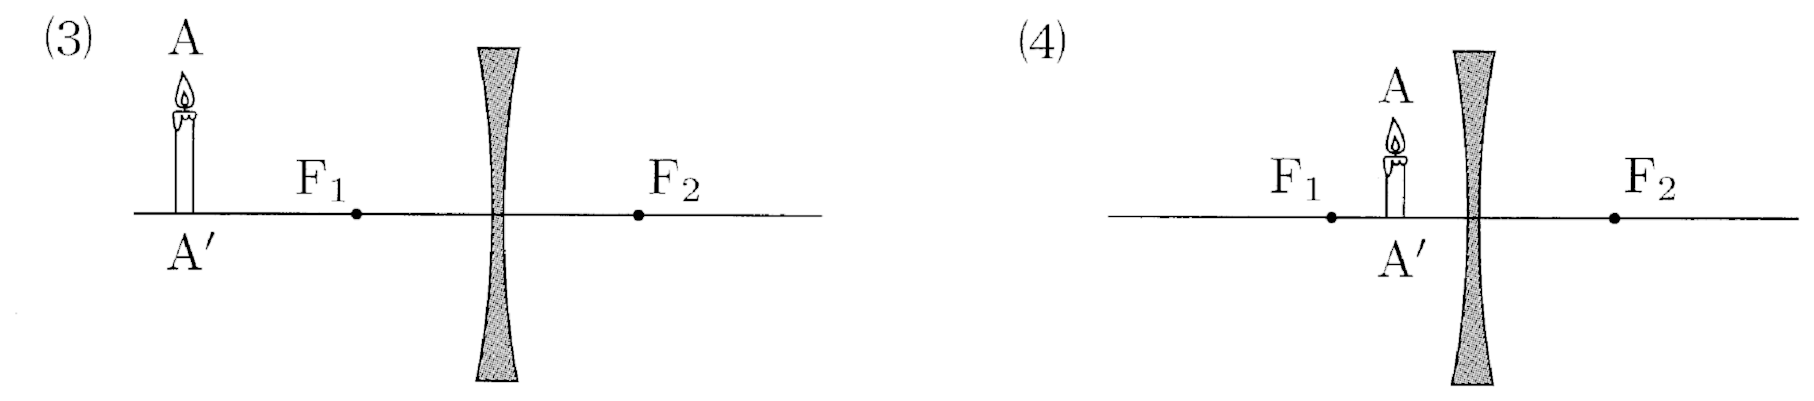
\includegraphics[keepaspectratio,width=128mm]{fig/n20_ex28b.png}
\end{center}
\end{reidai}

\begin{sisinE}
どの図についても，作図に使う光線は\MARU{1}〜\MARU{3}のうちの2本でよい．{\gtfamily 光軸に平行な光}と{\gtfamily レンズの中心を通る光}の2本を選ぶのが最も速い．

(2)と(4)は{\gtfamily 物体が焦点の内側にある}場合で，屈折光は交わらない．このときは{\gtfamily 屈折光を手前側へ延長して}交点を取り，そこに虚像が出来ると考える．虚像か実像かは「屈折した光そのものが集まるか，その延長が集まるか」で決まることを確認しておこう．
\end{sisinE}

\Key{凸レンズによる像の作図：\MARU{1} 光軸に平行に出た光　\MARU{2} レンズの中心を通過する光　\MARU{3} 手前側の焦点を通る光\\
\hspace*{1zw}凹レンズによる像の作図：\MARU{1} 光軸に平行に出た光　\MARU{2} レンズの中心を通過する光　\MARU{3} 向こう側の焦点へ直進する光\\
\hspace*{1zw}のうち，2つの光線の交点を作図する．}

\begin{kaitou}
\hspace{1zw}光軸に平行に入射する光と，レンズの中心を直進する光により，像の位置は次のように作図される（破線は屈折光の延長）．
\begin{center}
\AnaFig{128mm}{fig/n20_ex28_ans1.png}{fig/n20_ex28_blank1.png}\\[2mm]
\AnaFig{112mm}{fig/n20_ex28_ans2.png}{fig/n20_ex28_blank2.png}
\end{center}
\hspace{1zw}各像の種類は，順に
\Ana{(1)\ \text{倒立実像}\quad (2)\ \text{正立虚像}\quad (3)\ \text{正立虚像}\quad (4)\ \text{正立虚像}\Ans}
\end{kaitou}

\begin{chuu}
凸レンズでも{\gtfamily 物体が焦点の内側にあれば虚像}になる（(2)）．一方，凹レンズは物体の位置によらず，実光源に対しては{\gtfamily 必ず正立虚像}であり，しかも像は必ず物体より小さくなる（(3)(4)）．写像公式を学んだあとに，$f>0$と$f<0$の直角双曲線を描いて確かめておくとよい．
\end{chuu}
\end{reidaiunit}

\subsection{虚光源}

\begin{zuright}{70mm}
% 加筆（2026-09-20）：この1文は 20.2 の最後と同じ内容なので，復習であることを示した。
\hspace{1zw}20.2 で見たように，凹レンズに対し，レンズの向こう側にある焦点に光を集めるように凹レンズに光を入射すると，その光は凹レンズを通過した後，光軸に平行な光線群となる．

\hspace{1zw}ここで考えた，レンズの向こう側にある焦点に向かう光は，凹レンズよりも手前に凸レンズを置くことにより作ることができる．

\hspace{1zw}このように，レンズの向こう側にある一点に向かう光線群において，集光しようとしている場所を{\gtfamily 虚光源}と呼ぶ．
\zusep

\includegraphics[keepaspectratio,width=70mm]{text2_p19_fig1.png}
\end{zuright}

\hspace{1zw}光源，像の位置を次のように定義し直すと，虚光源や虚像もまとめて定義することができる．

\begin{matome}{光源と像}
\hspace{3mm}\MARU{1}\hspace{2mm}{\gtfamily 光源}\\
\hspace{5mm}{\gtfamily レンズに入射する直前の光線群（またはその延長）が一点に集まる場所．}光の進行方向に対して，その場所がレンズよりも手前ならば{\gtfamily 実光源}，レンズより奥ならば{\gtfamily 虚光源}となる．実際に光線群が光源の位置で集光しているかどうかは光源の位置を決定する上で関係がない．\\[1mm]
\hspace{3mm}\MARU{2}\hspace{2mm}{\gtfamily 像}\\
\hspace{5mm}{\gtfamily レンズにより屈折された直後の光線群（またはその延長）が一点に集まる場所．}光の進行方向に対して，その場所がレンズよりも奥ならば{\gtfamily 実像}，レンズより手前ならば{\gtfamily 虚像}となる．実際に光線群が像の位置で集光しているかどうかは像の位置を決定する上で関係がない．
\end{matome}

\begin{center}

\includegraphics[keepaspectratio,width=130mm]{text2_p19_fig2.png}
\end{center}

\hspace{1zw}レンズを通じて，入射する光が曲げられ，集光する位置が変化することを{\gtfamily 写像}と呼ぶ．光源，像は1回の写像ごとに位置が定義されるもので，特に複数のレンズを組み合わせた光学系では，各写像に対し，入射する光が実際に存在する光源から出た光であるとは限らず，また，レンズを通過した光が一点に集光するとは限らない．

%%%%% 例題29 ＝ 原本【例題29】〈レンズによる像〉（虚光源） %%%%%%%%%%%%%%%%%%%%
% 原本に解答図が無いので，解答図は TikZ で自作した（texify_draft/mkfig_new20ans.py）。
\bsNeed{80mm}
\begin{reidaiunit}
\begin{reidai}{レンズによる像}
% 加筆（2026-09-20）：この例題の $\mathrm{AA^\prime}$ はいずれも虚光源で，そこに物体が
% 置かれているわけではない（例題28の問題文をそのまま流用していた）ので言い換えた。
\hspace{1zw}焦点が$\mathrm{F_1}$, $\mathrm{F_2}$であるような凸レンズ，凹レンズがある．レンズに対して図のような位置に光源$\mathrm{AA^\prime}$（いずれも虚光源）があるとき，各図について光源$\mathrm{AA^\prime}$の像$\mathrm{BB^\prime}$を作図し，像の種類を述べよ．
\begin{center}
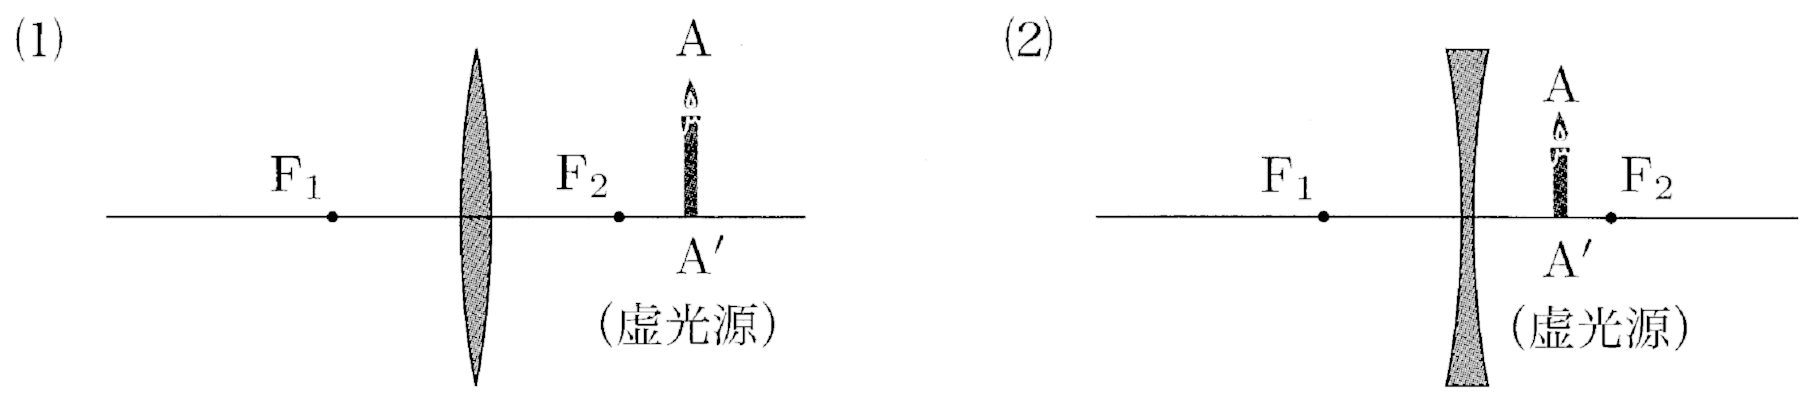
\includegraphics[keepaspectratio,width=128mm]{fig/n20_ex29a.png}\\[2mm]
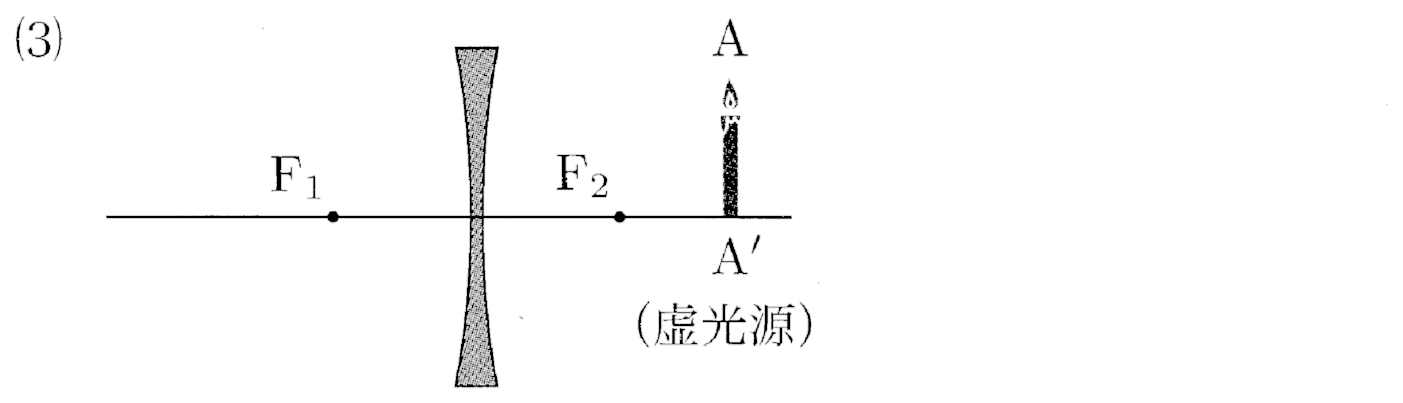
\includegraphics[keepaspectratio,width=99mm]{fig/n20_ex29b.png}
\end{center}
\end{reidai}

\begin{sisinE}
いずれも{\gtfamily 虚光源}の場合である．虚光源では「$\mathrm{A}$から光が出ている」のではなく，{\gtfamily $\mathrm{A}$に向かって光が集まってきている}のだから，入射光の向きを取り違えないこと．

作図に使う光線は実光源のときと同じ2本でよい．{\gtfamily 光軸に平行に入射する光}（屈折後は凸レンズなら$\mathrm{F_2}$を通り，凹レンズなら$\mathrm{F_1}$から出たように進む）と，{\gtfamily レンズの中心$\mathrm{O}$を通って$\mathrm{A}$へ向かう光}（曲がらずに直進する）の2本の，屈折後の光線の交点が像である．
\end{sisinE}

\Key{虚光源のときも作図の手順は変わらない．\MARU{1}光軸に平行な光，\MARU{2}レンズの中心を通る光，の\\
\hspace*{1zw}屈折後の2本の交点（交わらなければその延長の交点）が像である．}

\begin{kaitou}
\hspace{1zw}光軸に平行に入射する光と，レンズの中心を通って$\mathrm{A}$へ向かう光により，像の位置は次のように作図される（点線は入射光が$\mathrm{A}$に向かっていることを表す）．
\begin{center}
\AnaFig{128mm}{fig/n20_ex29_ans1.png}{fig/n20_ex29_blank1.png}\\[2mm]
\AnaFig{94mm}{fig/n20_ex29_ans2.png}{fig/n20_ex29_blank2.png}
\end{center}
\hspace{1zw}各像の種類は，順に
\Ana{(1)\ \text{正立実像}\quad (2)\ \text{正立実像}\quad (3)\ \text{倒立虚像}\Ans}
\end{kaitou}

\begin{chuu}
% 修正（2026-09-20）：加筆時の「逆に凸レンズでも…虚像になる場合がある」は誤り。
% 凸レンズ（$f>0$）に虚光源（$a<0$）を入れると $1/b=1/f+1/|a|>0$ で必ず $b>0$（実像）になる。
% 正しくは凹レンズ側の話（虚光源が焦点より遠ければ虚像＝設問(3)）なので書き直した。
凹レンズであっても，{\gtfamily 虚光源がレンズから焦点距離より近いところにあれば実像}が出来る（(2)）．逆に{\gtfamily 虚光源が焦点より遠ければ虚像}になる（(3)）．一方，{\gtfamily 凸レンズは虚光源に対しては必ず実像}を作る（(1)）．「凸レンズだから実像」「凹レンズだから虚像」という覚え方は虚光源では通用しない．写像公式（次節）に$a<0$を代入すれば，これらはすべて機械的に確かめられる．
\end{chuu}
\end{reidaiunit}

\subsection{凹面鏡・凸面鏡}

% 原本は「光の集光，写像を議論することが出来る」。旧 physics_ch27.tex は「五輪する」と
% 誤入力されていたので直した（2026-09-10）。
\hspace{1zw}鏡によっても，光の集光，写像を議論することが出来る．中央部がへこんでいる鏡を{\gtfamily 凹面鏡}，出っ張っている鏡を{\gtfamily 凸面鏡}と呼ぶ．

\hspace{1zw}凹面鏡に光軸に対して平行な光線を当てると，反射光は鏡の手前のある一点に集光する．この点を凹面鏡の{\gtfamily 焦点}と呼び，凹面鏡から焦点までの距離を焦点距離と呼ぶ．また，焦点の位置に光源を置くと，光線の通り道は先ほどと逆になり，反射光は光軸と平行な光線群となる．

\hspace{1zw}凸面鏡に光軸に対して平行な光線を当てると，反射光は広がっていき，その光線を凸面鏡の奥側まで伸ばすと，直線は一点で交わる．この位置を凸面鏡の{\gtfamily 焦点}と呼び，凸面鏡から焦点までの距離を焦点距離と呼ぶ．また，凸面鏡の奥側の焦点に集まるような光線を入射すると，反射光は光軸と平行な光線群となる．

\begin{center}

\includegraphics[keepaspectratio,width=130mm]{text2_p21_fig1.png}
\end{center}

% 原本には無いが，作図の要点（練習［65］に必要）をまとめ枠として加筆した（2026-09-10）。
\begin{matome}{鏡による像の作図}
\hspace{3mm}\MARU{1} 鏡に{\gtfamily 光軸と平行に入射する光}は，凹面鏡では{\gtfamily 手前側の}，凸面鏡では{\gtfamily 奥側の}焦点を通る直線となるように反射される．\\
\hspace{3mm}\MARU{2} {\gtfamily 鏡の中央に入射する光}は，入射角と反射角が等しくなるよう，平面鏡で反射された場合と同じように反射される．\\[1mm]
\hspace{3mm}結果的に，{\gtfamily 凹面鏡による結像は凸レンズによる結像を，凸面鏡による結像は凹レンズによる結像を，それぞれ反射面（レンズの位置）に関して折り返したもの}と同じになる．
\end{matome}

% 原本の本文には平面鏡による像の説明が無いが，練習［69］［74］はこれを使う（2026-09-10 加筆）。
\hspace{1zw}なお，{\gtfamily 平面鏡}は「焦点距離が無限大の球面鏡」とみなすことができる．平面鏡に当たった光は，入射角と反射角が等しくなるように反射されるので，反射光は{\gtfamily 鏡面に関して光源と対称な位置から出てきたかのように}進む．すなわち，平面鏡は物体と鏡面に関して対称な位置に，物体と同じ大きさの正立の虚像を作る．

\begin{matome}{平面鏡による像}
\hspace{3mm}平面鏡は，{\gtfamily 物体（光源）と鏡面に関して対称な位置}に，{\gtfamily 同じ大きさの正立の虚像}を作る．\\
\hspace{3mm}したがって，レンズと平面鏡を組み合わせた光学系では，「レンズによる像の位置を鏡面で折り返した点」が，次にレンズへ入る光にとっての光源の位置になる．
\end{matome}

\subsection{写像公式}

\hspace{1zw}作図した図を元に，光源の位置と像の位置に関する関係式を導くことが出来る．

\begin{zuright}{80mm}
\hspace{1zw}まず，右図のような凸レンズの写像について考えてみよう．

\hspace{1zw}この図において，レンズの焦点距離を$f\U{m}$，レンズから光源までの距離を$a\U{m}$，レンズから実像までの距離を$b\U{m}$とすると，$\triangle\mathrm{AA^\prime O}\backsim\triangle\mathrm{BB^\prime O}$，また$\triangle\mathrm{POF_2}\backsim\triangle\mathrm{BB^\prime F_2}$であるから，
\zusep

\includegraphics[keepaspectratio,width=80mm]{text2_p22_fig1.png}
\end{zuright}
\[\frac{\mathrm{AA^\prime}}{\mathrm{BB^\prime}}=\frac{a}{b}\hspace{4mm},\hspace{4mm}\frac{\mathrm{PO}}{\mathrm{BB^\prime}}=\frac{f}{b-f}\]
% 加筆（2026-09-20）：PO＝AA' であることが書かれておらず，原本の式変形
% 「$\mathrm{PO}/\mathrm{BB^\prime}=\mathrm{AA^\prime}/\mathrm{BB^\prime}$」がなぜ成り立つのか読めなかった。
が成立する．ここで$\mathrm{P}$は{\gtfamily 光軸に平行に進んできた光線がレンズに入る点}であり，その高さは光源の高さに等しいから$\mathrm{PO}=\mathrm{AA^\prime}$である．よって上の2式の左辺どうしが等しく，これを整理すると，
\[\frac{a}{b}=\frac{f}{b-f}\ \Longleftrightarrow\ a(b-f)=bf\ \Longleftrightarrow\ bf+af=ab\ \Longleftrightarrow\ \frac{1}{a}+\frac{1}{b}=\frac{1}{f}\]
が得られる．

\begin{zuright}{78mm}
\hspace{1zw}凹レンズの写像についても考えてみよう．図において，レンズの焦点距離を$f\U{m}$，レンズから光源までの距離を$a\U{m}$，レンズから虚像までの距離を$b\U{m}$とすると，$\triangle\mathrm{AA^\prime O}\backsim\triangle\mathrm{BB^\prime O}$，また$\triangle\mathrm{POF_1}\backsim\triangle\mathrm{BB^\prime F_1}$であるから，
\[\frac{\mathrm{AA^\prime}}{\mathrm{BB^\prime}}=\frac{a}{b}\hspace{3mm},\hspace{3mm}\frac{\mathrm{PO}}{\mathrm{BB^\prime}}=\frac{f}{f-b}\]
が成立する．凸レンズのときと同様に$\mathrm{PO}=\mathrm{AA^\prime}$である．
\zusep

\includegraphics[keepaspectratio,width=78mm]{text2_p22_fig2.png}
\end{zuright}

\hspace{1zw}これを整理すると，
\[\frac{a}{b}=\frac{f}{f-b}\ \Longleftrightarrow\ a(f-b)=bf\ \Longleftrightarrow\ bf-af=-ab\ \Longleftrightarrow\ \frac{1}{a}-\frac{1}{b}=-\frac{1}{f}\]
が得られる．この式は，凸レンズにおける式において，$b$および$f$の符号が逆になっている．

\hspace{1zw}これらの結果は，像の位置$b$，焦点距離$f$を次のように設定し直すことで，1つの式にまとめて表すことが出来る．

\begin{description}
\item[\MARU{1}] {\gtfamily 像の位置 \mbox{\boldmath$b$}}\\
レンズの位置を原点に{\gtfamily レンズの向こう側を正として}$b$軸を取る．つまり，{\gtfamily 実像となる場合に$b>0$，虚像となる場合に$b<0$}となるように定める．
\item[\MARU{2}] {\gtfamily 焦点距離 \mbox{\boldmath$f$}}\\
{\gtfamily 凸レンズの場合に$f>0$，凹レンズの場合に$f<0$}となるように取る．平行光を入射した際の像の位置$b$として定めていると考えることが出来る．
\end{description}

\hspace{1zw}さらに，光源の位置が虚光源となる場合であっても，同様に三角形の相似を考えることで同じ関係式が得られる．そこで，光源の位置$a$についても

\begin{description}
\item[\MARU{3}] {\gtfamily 光源の位置 \mbox{\boldmath$a$}}\\
レンズの位置を原点に{\gtfamily レンズの手前側を正として}$a$軸を取る．つまり，{\gtfamily 実光源となる場合に$a>0$，虚光源となる場合に$a<0$}となるように定める．
\end{description}

\hspace{1zw}と定めれば，実光源・虚光源，実像・虚像，凸レンズ・凹レンズのすべての場合が1つの式でまとめられる．

\begin{matome}{写像公式}
\hspace{3mm}レンズから光源までの距離$a\U{m}$はレンズの手前側を正に，レンズから像までの距離$b\U{m}$はレンズの向こう側を正に取り，焦点距離$f\U{m}$は凸レンズのときを正，凹レンズのときを負に取る（{\gtfamily $a$, $b$, $f$ はいずれも符号つきの量で，負の値も取りうる}）と，次の写像公式が成立する．
\[\frac{1}{a}+\frac{1}{b}=\frac{1}{f}\]
\hspace*{20mm}$a>0$：実光源\hspace{12mm}$b>0$：実像\\
\hspace*{20mm}$a<0$：虚光源\hspace{12mm}$b<0$：虚像\\[1mm]
\hspace{3mm}また，像の大きさは光源の大きさに比べて$\left|\ \dfrac{b}{a}\ \right|$倍となる．これを{\gtfamily 倍率}と呼ぶ．
\end{matome}

% 原本の本文には「像の向きの判定」と「写像公式の直角双曲線」が無いが，
% 例題30の（指針）・練習［72］(2)・練習［75］(2) はこれを前提にしている（2026-09-10 加筆）。
\hspace{1zw}倍率は絶対値で定義したが，{\gtfamily 像が正立か倒立かは$\dfrac{b}{a}$の符号で決まる}．作図で確かめると分かるように，光源と像が{\gtfamily レンズをはさんで反対側}にある（$a$と$b$が同符号の）ときは像が上下逆になり，{\gtfamily レンズから見て同じ側}にある（異符号の）ときは像の向きが変わらない．

\hspace{1zw}また，写像公式$\dfrac{1}{a}+\dfrac{1}{b}=\dfrac{1}{f}$は，両辺に$ab f$を掛けて整理すると
\[(a-f)(b-f)=f^2\]
と変形できる．これは$a$--$b$平面上で，$a=f$と$b=f$を漸近線とする{\gtfamily 直角双曲線}を表す．この曲線を描いておくと，「光源をどこに置くとどんな像が出来るか」が一目で分かるので，計算する前に必ず描く習慣をつけたい．

\begin{center}
% 本文では特定の問題の点を指していないので，● の無い図を使う（2026-09-20）。
\raisebox{-0.5\height}{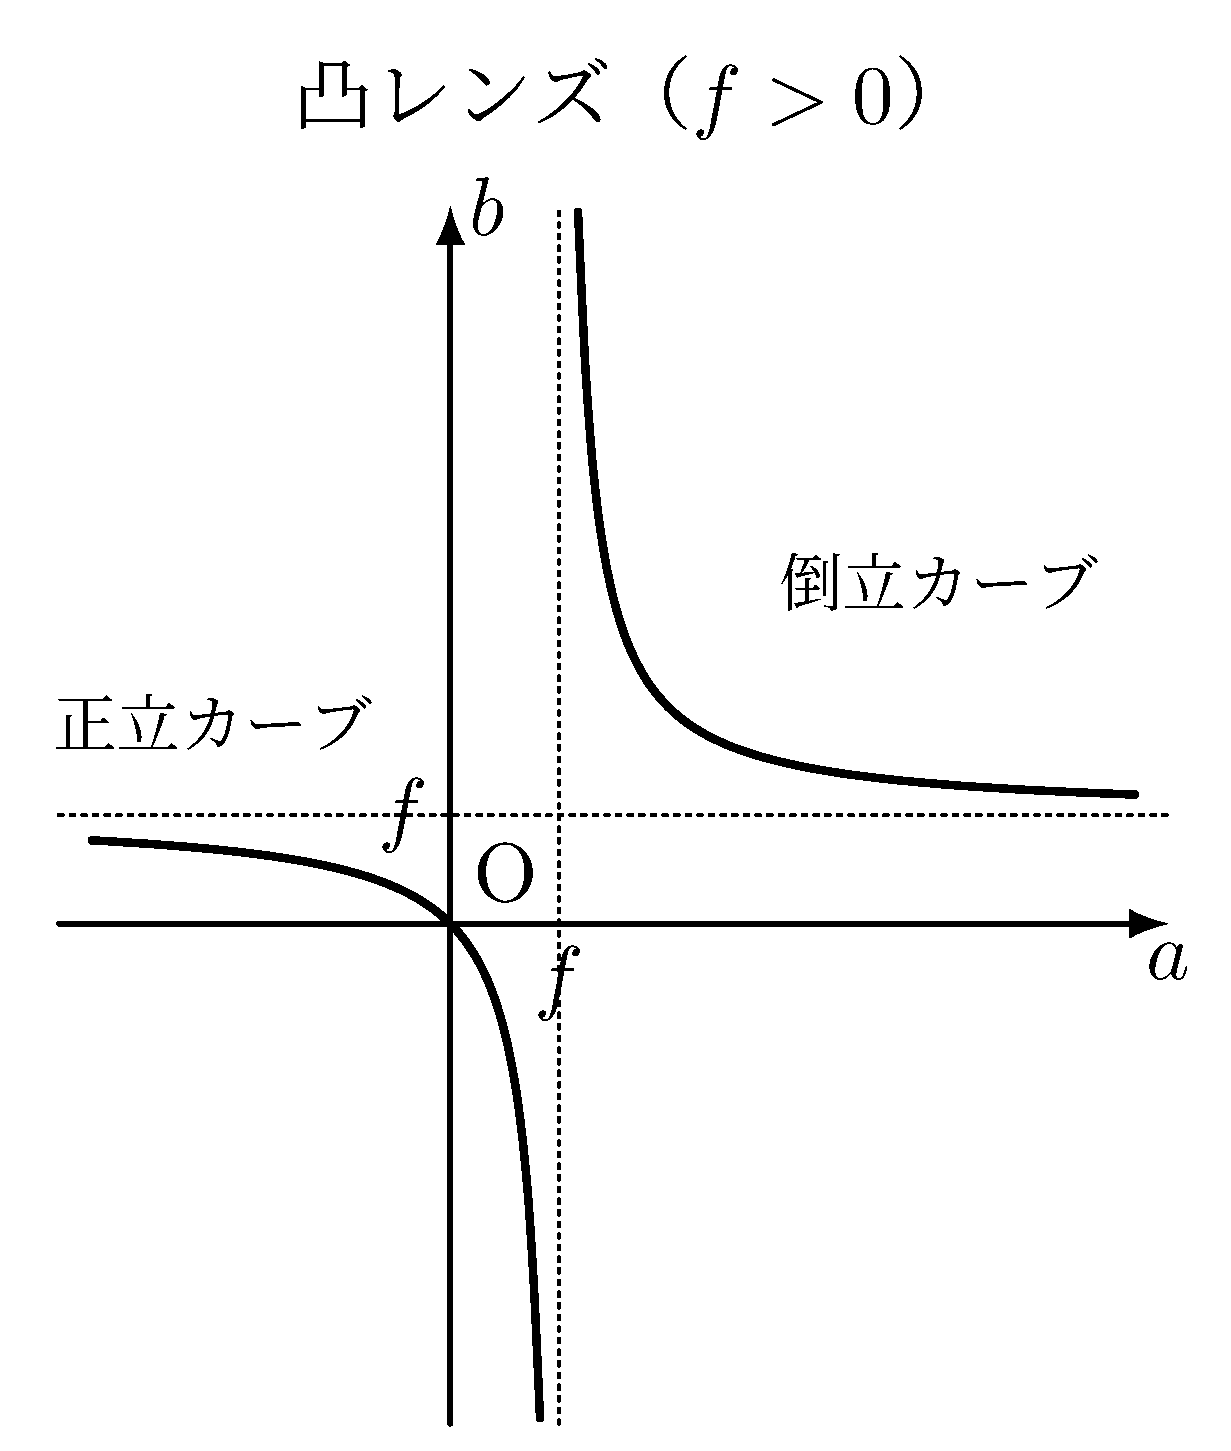
\includegraphics[keepaspectratio,width=62mm]{fig/n20_hyp_conv.png}}\hspace{4mm}%
\raisebox{-0.5\height}{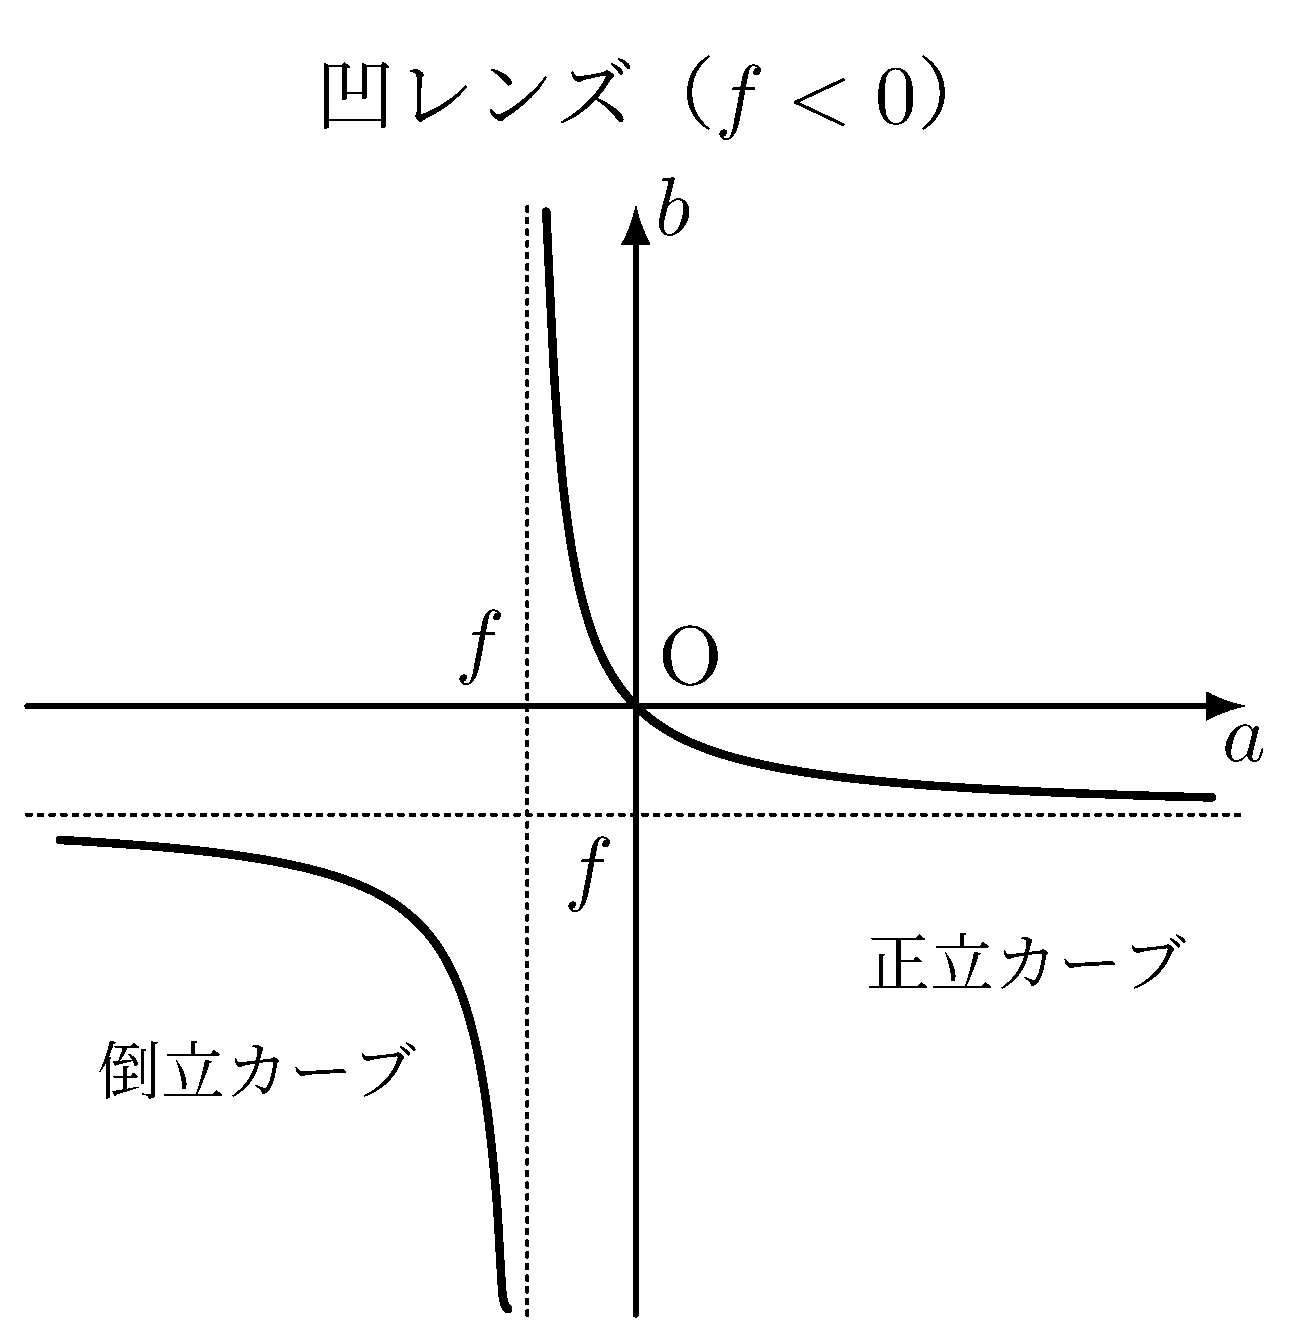
\includegraphics[keepaspectratio,width=62mm]{fig/n20_hyp_conc.png}}
\end{center}

\begin{matome}{像の向きの判定}
\hspace{3mm}\MARU{1} $\dfrac{b}{a}>0$（光源と像がレンズをはさんで反対側）のとき　{\gtfamily 倒立像}\\
\hspace{3mm}\MARU{2} $\dfrac{b}{a}<0$（光源と像がレンズから見て同じ側）のとき　{\gtfamily 正立像}\\[1mm]
\hspace{3mm}直角双曲線$(a-f)(b-f)=f^2$の上では，{\gtfamily 凸レンズ（$f>0$）は右上のカーブが倒立像・左下のカーブが正立像}，{\gtfamily 凹レンズ（$f<0$）は右上のカーブが正立像・左下のカーブが倒立像}にあたる．
\end{matome}

%%%%% 例題30 ＝ 原本【例題30】〈レンズの写像公式〉 %%%%%%%%%%%%%%%%%%%%%%%%%%%%
% 図（直角双曲線）は㉘[68]の解答（prob2_p87）から切り出した。
\bsNeed{56mm}
\begin{reidaiunit}
\begin{reidai}{レンズの写像公式}
\hspace{1zw}凸レンズおよび凹レンズを用いて次のように物体を置くとき，出来る像の位置および倍率を求めよ．また，それは実像と虚像のいずれか．さらに，それは正立像，倒立像のいずれか．
\begin{komon}
\ko{1} 焦点距離$8.0\U{cm}$の凸レンズの光軸上，レンズの手前側$10\U{cm}$の位置にロウソクを置くとき．
\ko{2} 焦点距離$4.0\U{cm}$の凹レンズの光軸上，レンズの手前側$6.0\U{cm}$の位置にロウソクを置くとき．
\end{komon}
\end{reidai}

\begin{sisinE}
写像公式$\dfrac{1}{a}+\dfrac{1}{b}=\dfrac{1}{f}$を用いて，まず像の座標を計算し，続いて倍率公式$m=\left|\dfrac{b}{a}\right|$で倍率を求めよう．実像・虚像のいずれであるかは$b$の正負で分かる．すなわち，$b>0$のときはレンズの向こう側で光が収束するので実像が出来ており，$b<0$の場合はレンズの手前側から光が直進したかのように進んでいるのだから虚像が出来ることになる．

正立像か倒立像かは簡単な図を描いて判定するか，もしくは{\gtfamily 直角双曲線$(a-f)(b-f)=f^2$}において，\MARU{1}凸レンズの場合は右上のカーブが倒立像のカーブ，左下のカーブが正立像のカーブ，\MARU{2}凹レンズの場合は右上のカーブが正立像のカーブ，左下のカーブが倒立像のカーブであることを利用して判定する．
\end{sisinE}

\Key{写像公式\hspace{3mm}$\dfrac{1}{a}+\dfrac{1}{b}=\dfrac{1}{f}$\hspace{8mm}倍率\hspace{3mm}$m=\left|\dfrac{b}{a}\right|$}

\begin{kaitou}
\begin{komon}
\ko{1} 凸レンズであるから$f=+8.0\U{cm}$，実光源であるから$a=+10\U{cm}$とおいて写像公式に当てはめると，
       \Ana{\frac{1}{10}+\frac{1}{b}=\frac{1}{8.0}\quad\text{より}\quad b=+40\U{cm}\ (>0)}
       である．すなわち，レンズの向こう側の$\AnaU{40}\U{cm}$の位置に
       \Ana{m=\left|\frac{b}{a}\right|=4.0\ \text{倍}}
       の倍率の実像が出来る．また，$\dfrac{1}{a}+\dfrac{1}{b}=\dfrac{1}{f}$を変形すると$(a-f)(b-f)=f^2$となり，次図のような直角双曲線が得られる．いま求めた$(a,\,b)$は図の$\bullet$の点に対応しているので，これは\AnaU{\gtfamily 倒立像}であることが分かる．
       \begin{center}\AnaFig{66mm}{fig/n20_ex30_conv.png}{fig/n20_ex30_conv_blank.png}\end{center}
       \Ana{\text{レンズの向こう側}\ 40\U{cm}\ \text{の位置に，倍率}\ 4.0\ \text{倍の倒立実像}\Ans}
\ko{2} 凹レンズであるから$f=-4.0\U{cm}$，実光源であるから$a=+6.0\U{cm}$とおいて写像公式に当てはめると，
       \Ana{\frac{1}{6.0}+\frac{1}{b}=\frac{1}{-4.0}\quad\text{より}\quad b=-2.4\U{cm}}
       である．すなわち，レンズの手前側の$\AnaU{2.4}\U{cm}$の位置に
       \Ana{m=\left|\frac{b}{a}\right|=0.4\ \text{倍}}
       の倍率の虚像が出来る．また，次図のような写像公式の直角双曲線のカーブを考えるとこれは図の$\bullet$の点に対応しているので，\AnaU{\gtfamily 正立像}であることが分かる．
       \begin{center}\AnaFig{66mm}{fig/n20_ex30_conc.png}{fig/n20_ex30_conc_blank.png}\end{center}
       \Ana{\text{レンズの手前側}\ 2.4\U{cm}\ \text{の位置に，倍率}\ 0.4\ \text{倍の正立虚像}\Ans}
\end{komon}
\end{kaitou}
\end{reidaiunit}

%%%%% 例題31 ＝ 原本【例題31】〈複合レンズ〉 %%%%%%%%%%%%%%%%%%%%%%%%%%%%%%%%%%
\bsNeed{40mm}
\begin{reidaiunit}
\begin{reidai}{複合レンズ}
\hspace{1zw}焦点距離$f_1\U{m}$, $f_2\U{m}$の2つの凸レンズを，光軸を合わせて密着させた．この合わせレンズの焦点距離を求めよ．
\end{reidai}

\begin{sisinE}
この合わせレンズに平行光を入射したとき，集光される場所を求めればよい．1つ目のレンズのみであれば，レンズから$f_1\U{m}$の位置に集光されるので，2つ目のレンズにとっては，{\gtfamily この場所が虚光源となっている写像}となる．
\end{sisinE}

\Key{合わせレンズの焦点距離$f$は\hspace{3mm}$\dfrac{1}{f}=\dfrac{1}{f_1}+\dfrac{1}{f_2}$}

\begin{kaitou}
\hspace{1zw}合わせレンズに光軸に平行な光を入射する．2枚は十分に薄く密着しているので，レンズの位置は同一とみなしてよい．

\hspace{1zw}1枚目のレンズだけを考えると，平行光は無限に遠い光源から来た光とみなせるので$a_1=\infty$，すなわち$\dfrac{1}{a_1}=0$である．写像公式より
\Ana{\frac{1}{\infty}+\frac{1}{b_1}=\frac{1}{f_1}\quad\text{より}\quad b_1=f_1\U{m}}
すなわちレンズの向こう側$f_1\U{m}$の位置に集光しようとする．

\hspace{1zw}この光がそのまま2枚目のレンズに入射するので，2枚目のレンズにとっては，レンズの向こう側$f_1\U{m}$の位置が光源，すなわち{\gtfamily 虚光源}である．したがって$a_2=-f_1\U{m}$として写像公式を適用すると，
\Ana{\frac{1}{-f_1}+\frac{1}{b_2}=\frac{1}{f_2}\quad\text{より}\quad b_2=\frac{f_1f_2}{f_1+f_2}\U{m}}

\hspace{1zw}合わせレンズに平行光を入射したときに集光する位置が合わせレンズの焦点であるから，求める焦点距離$f$は
\Ana{f=b_2=\frac{f_1f_2}{f_1+f_2}\U{m}\quad\left(\text{すなわち}\ \frac{1}{f}=\frac{1}{f_1}+\frac{1}{f_2}\right)\Ans}
\end{kaitou}

\begin{chuu}
$\dfrac{1}{f}$は{\gtfamily レンズの度}（ジオプトリー）と呼ばれ，密着したレンズでは単純に足し算になる．凹レンズを密着させる場合も$f<0$として同じ式が使えるので，たとえば焦点距離の等しい凸レンズと凹レンズを密着させると$\dfrac{1}{f}=\dfrac{1}{f_1}-\dfrac{1}{f_1}=0$，すなわち$f=\infty$となり，光を曲げない（ただのガラス板と同じ）ことが分かる．
\end{chuu}
\end{reidaiunit}

\subsection{偏光}

\begin{zuright}{54mm}
\hspace{1zw}光は横波であるため，進行方向に対して垂直な面内で振動しているが，太陽の光などは垂直な面内のあらゆる方向に振動しており，ある特定の方向のみに偏って振動してはいない．このような光を{\gtfamily 自然光}と呼ぶ．

\hspace{1zw}しかし，{\gtfamily 偏光板}と呼ばれる板を用意してこれに自然光を通すと，偏光板を通過した光はある特定の方向のみの振動になり，それに垂直な方向の振動は全くなくなる．このように，ある特定方向のみの振動となったものを{\gtfamily 偏光}と呼ぶ．

\hspace{1zw}この現象は，偏光板を一種のブラインドのようなものだと考えると分かりやすい．ブラインドの筋目に沿った方向の振動を持つ光はこれを通過することができるが，それに垂直な方向の振動は通過することができない．そのため，2つの偏光板を用意してこれを順番に並べて光を通す場合，2つの偏光板の軸方向が揃っている場合は偏光は2枚目の偏光板を通過できるが，2つの偏光板の軸方向が互いに垂直になっている場合は偏光は2枚目の偏光板を通過できない．
\zusep

\includegraphics[keepaspectratio,width=48mm]{text2_p25_fig1.png}
\end{zuright}

\hspace{1zw}もし仮に光が縦波であるならこのような偏光という現象は起きないはずである．すなわち，{\gtfamily 偏光という現象は光波が横波であることを裏付ける1つの証拠}なのである．

% 原本の本文には分散・散乱の説明が無いが，練習［63］(3)(4) がこれを問う（2026-09-10 加筆）。
\hspace{1zw}最後に，身のまわりで見られる光の現象のうち，ここまでに扱っていない{\gtfamily 分散}と{\gtfamily 散乱}についてまとめておく．

\begin{matome}{分散と散乱}
\hspace{3mm}\MARU{1}\hspace{2mm}{\gtfamily 分散}\\
\hspace{5mm}物質の屈折率は，光の波長によってわずかに異なる（一般に{\gtfamily 波長の短い光ほど屈折率が大きい}）．そのため，白色光を物質に入射させると波長ごとに屈折角が異なり，光が色に分かれる．この現象を{\gtfamily 光の分散}といい，分かれた色の帯（光を波長ごとに分けて並べたもの）を{\gtfamily スペクトル}という．屈折率の大きい物質ほど分散の程度も大きく，ダイヤモンド（屈折率約2.4）がガラス（約1.5）よりも美しく色づいて見えるのはこのためである．プリズムで白色光が虹色に分かれるのも，雨上がりに虹が見えるのも分散による．\\[1mm]
\hspace{3mm}\MARU{2}\hspace{2mm}{\gtfamily 散乱}\\
\hspace{5mm}光が，波長に比べて小さい微粒子に当たると，進行方向以外のさまざまな向きへ散っていく．この現象を{\gtfamily 光の散乱}という．{\gtfamily 波長の短い光ほど散乱されやすい}ので，昼間の空は散乱された青い光で青く見える．一方，朝日や夕日は大気中を長く通ってくるため，散乱されやすい青い光が途中で失われ，散乱されにくい赤い光が多く残るので赤く見える．
\end{matome}

\newpage

% 練習番号：第14〜19回の練習題数の合計は 10+10+8+14+11+9＝62題．よって第20回は［63］から．
% ［63］は 原本㉘[69]〈光の現象〉．㉗[60][61]・㉘[68] は例題26・27・30 と同一問題なので
% A問題4題を1題に統合した（再編案の「A4→1」）。設問は1つも失われていない。
\setcounter{qno}{62}

\filbreak
\Rank{A問題}

\Mon{光の現象}

\hspace{1zw}次の光に関する現象と最も関係の深い用語を以下の語群\MARU{1}〜\MARU{4}の中から選べ．
\begin{komon}
\ko{1} 店のショーウィンドウのガラスに光が反射して中がよく見えないとき，サングラスをかけるとよく見える．
\ko{2} コンパクトディスクは美しく色づいて見える．
\ko{3} 朝日や夕日が赤く見える．
\ko{4} ダイヤモンドが美しく色づいて見える．
\end{komon}
\begin{center}
\fbox{\parbox{140mm}{\vspace{1mm}\hspace{1zw}【語群】\hspace{4mm}\MARU{1}\ 分散\hfill\MARU{2}\ 回折格子\hfill\MARU{3}\ 偏光\hfill\MARU{4}\ 散乱\hspace{4mm}\vspace{1mm}}}
\end{center}

\filbreak
\Rank{B問題}

\Mon[\Sitei]{レンズによる像の作図}

\hspace{1zw}各図において，光源の位置が以下のように与えられている（白黒反転しているものは虚光源であるとする）とき，レンズによる像の位置を作図せよ．また，像の種類（倒立か正立か，実像か虚像か）を答えよ．光は全て左から右に進んでいるものとする．ただし，図中の点は，各レンズから焦点距離分離れた位置を表している．
\begin{center}
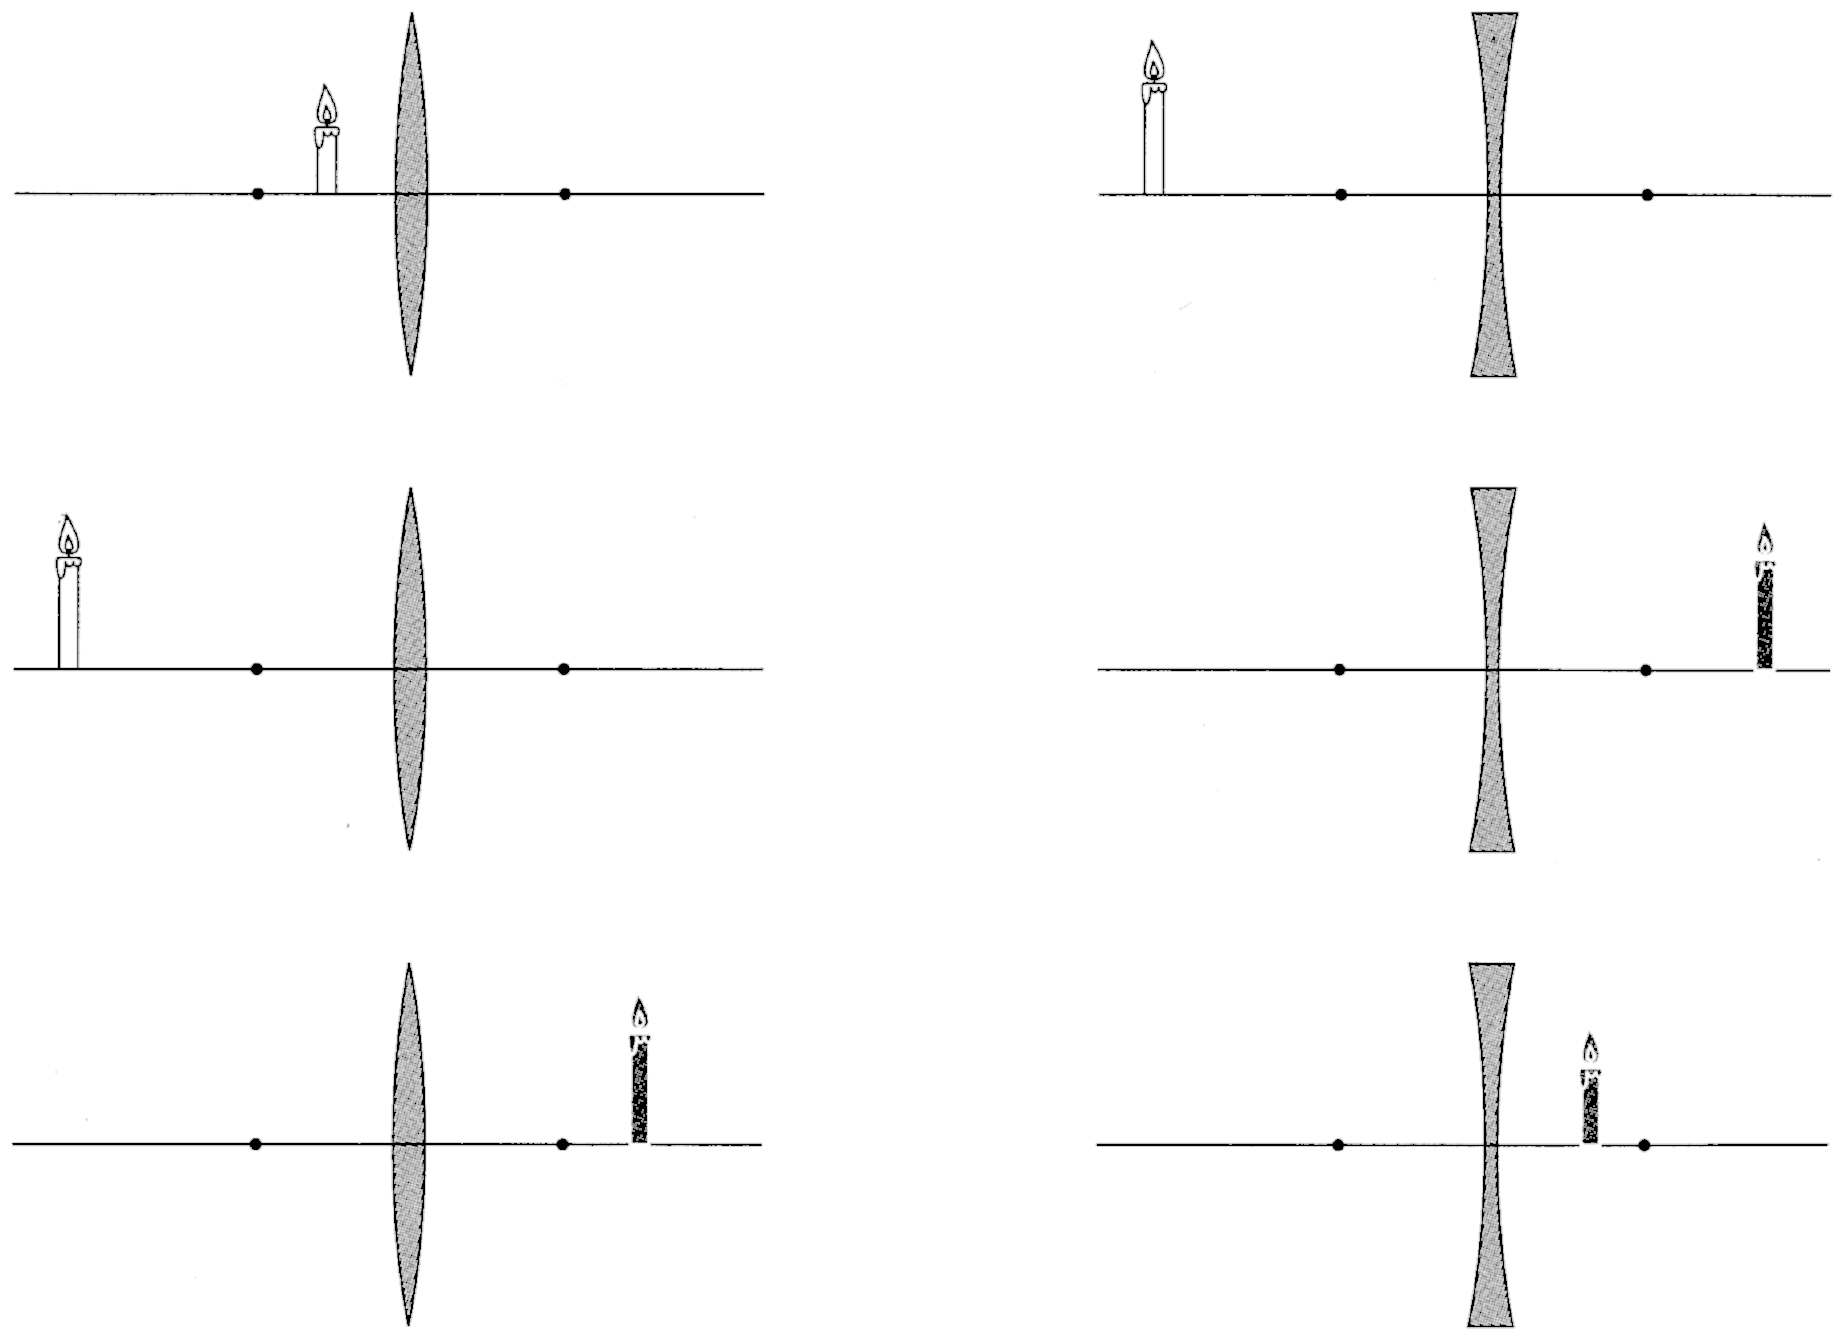
\includegraphics[keepaspectratio,width=130mm]{fig/n20_p64_zu.png}
\end{center}

\Mon{鏡による像の作図}

\hspace{1zw}各図において，光源の位置が以下のように与えられている（白黒反転しているものは虚光源であるとする）とき，鏡による像の位置を作図せよ．また，像の種類（倒立か正立か，実像か虚像か）を答えよ．光は全て左から右に進んでいるものとする．ただし，図中の点は，各鏡から焦点距離分離れた位置を表している．
\begin{center}
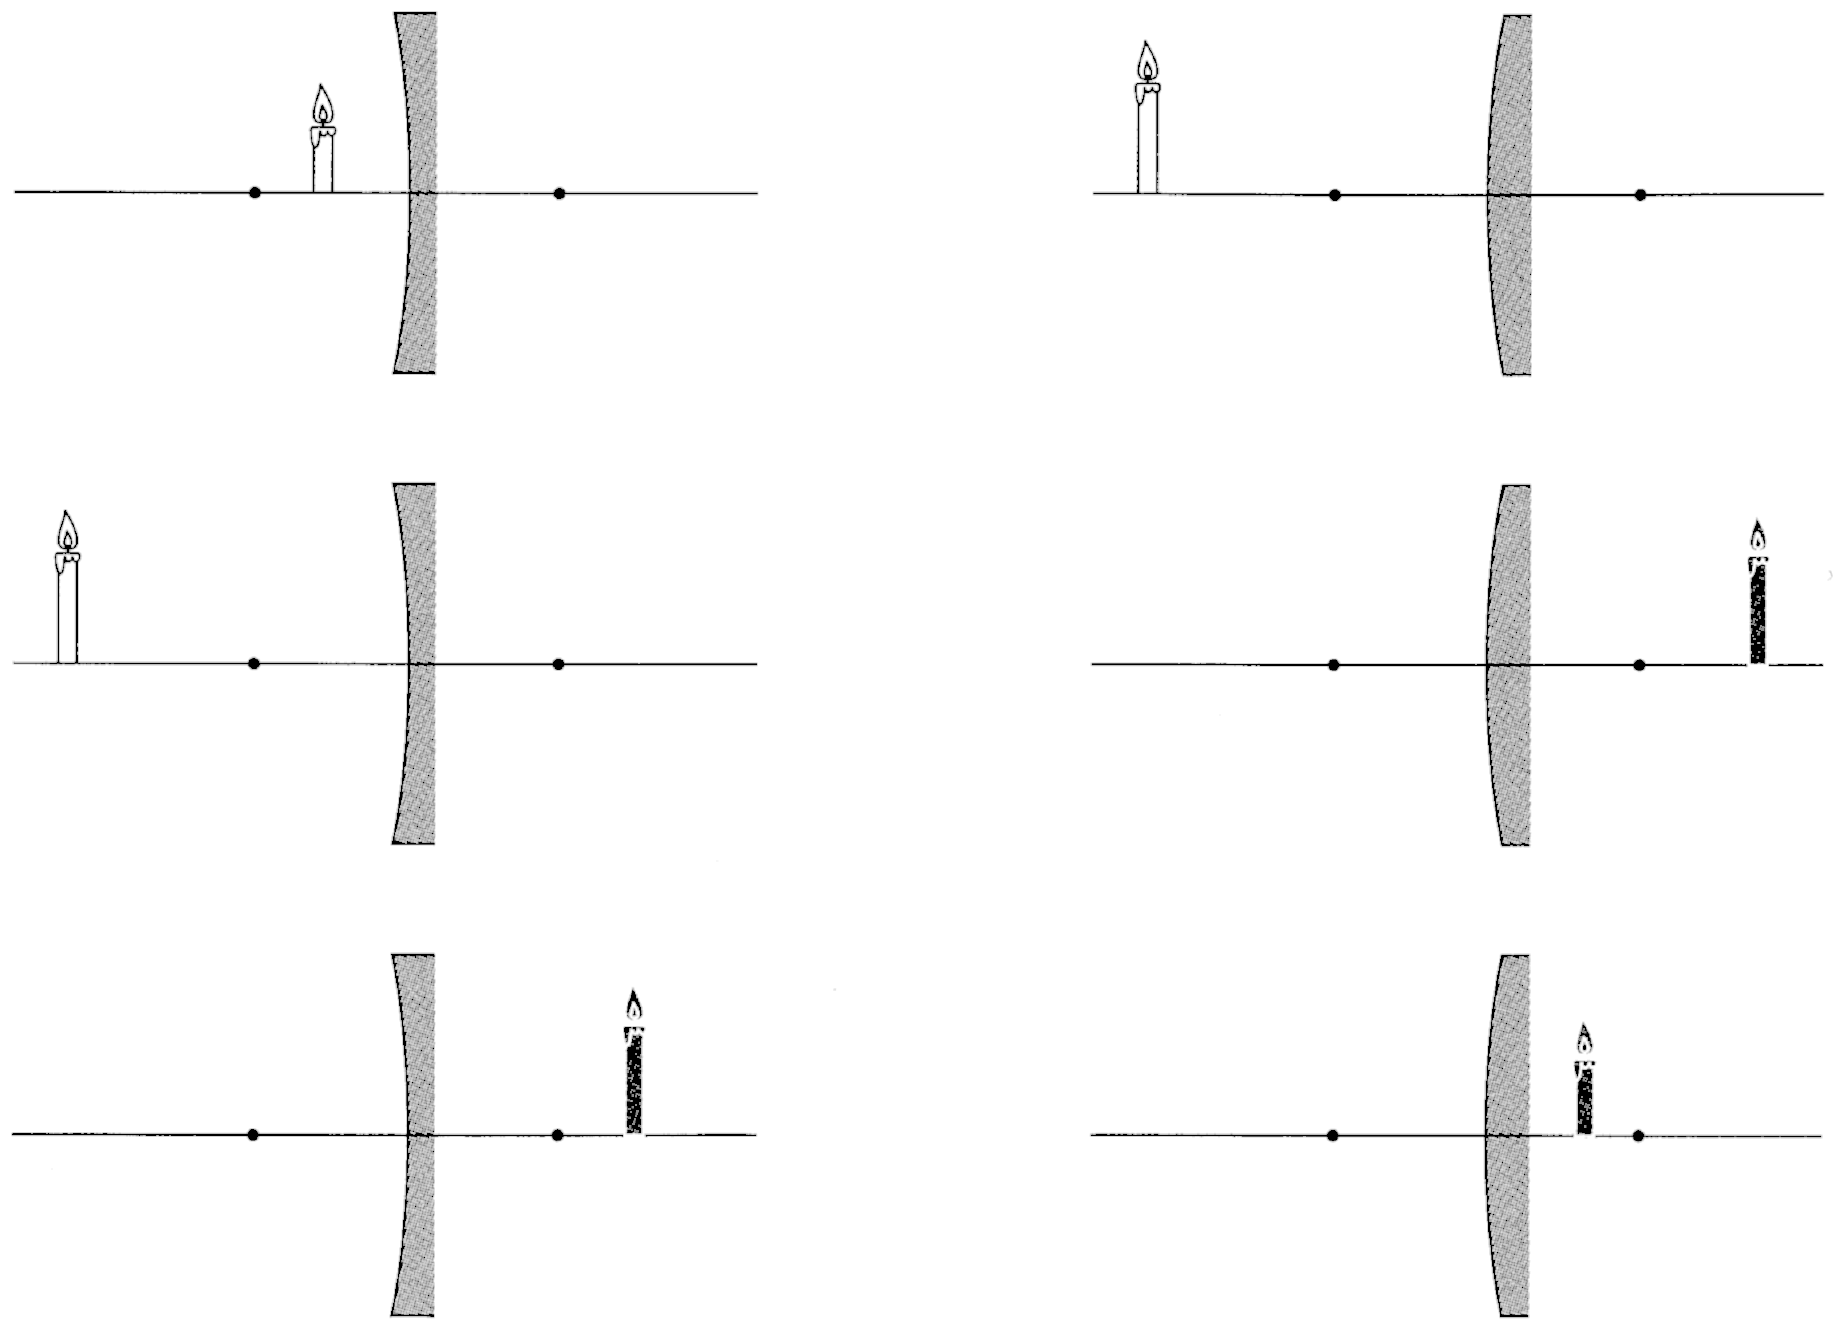
\includegraphics[keepaspectratio,width=130mm]{fig/n20_p65_zu.png}
\end{center}

\Mon[\Sitei]{近軸近似}

\begin{zuright}{76mm}
\hspace{1zw}片面が平面で，もう片面が半径$R$の球面になっているレンズの焦点距離について考える．右図のようにレンズをおき，レンズの光軸と平行に光を入射する．入射光の光軸からの距離を$z$，球面の中心を$\mathrm{O}$とし，空気の屈折率を1，レンズの屈折率を$n$とし，右図のように点$\mathrm{A}$, $\mathrm{B}$, $\mathrm{P}$をとったとき，以下の問いに答えよ．
\zusep
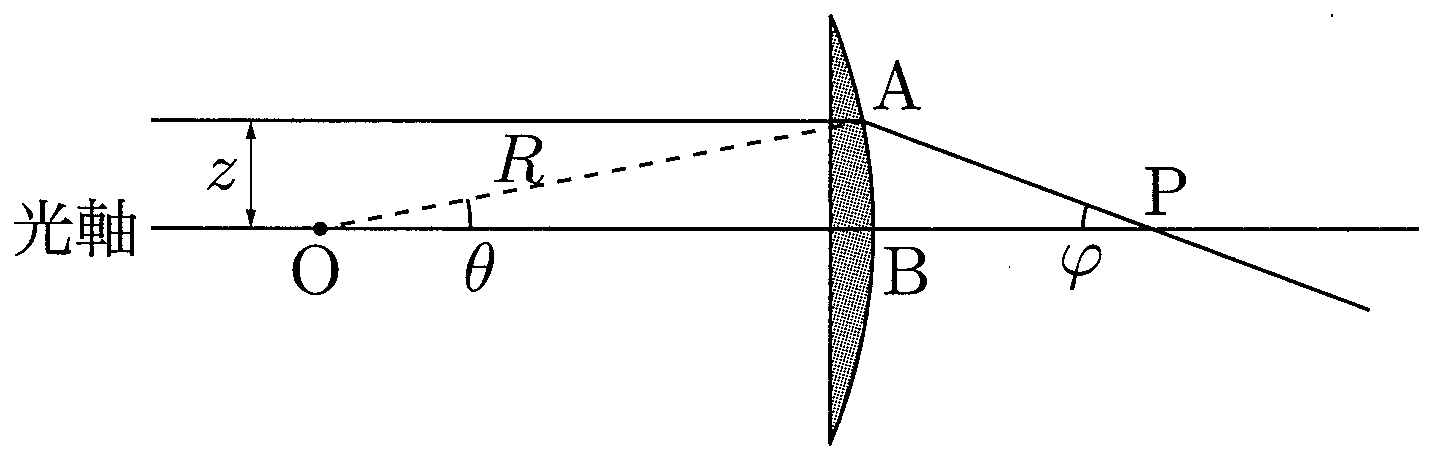
\includegraphics[keepaspectratio,width=76mm]{fig/n20_p66_zu.png}
\end{zuright}
\begin{komon}
\ko{1} $\angle\mathrm{AOB}=\theta$, $\angle\mathrm{APB}=\varphi$としたとき，点$\mathrm{A}$における屈折から，$\theta$と$\varphi$の関係式を求めよ．
% 修正（2026-09-20）：原本（prob2_p12 の[64]）は2箇所とも「$z\leqq R$」だが，
% $z=R$ なら $\theta=90^\circ$ で微小ではないので「$z\ll R$」の誤植と判断して直した。
\ko{2} $z\ll R$のとき，$\theta$, $\varphi$は微小であるとしてよい．$x$が微小なとき$x\fallingdotseq\sin x\fallingdotseq\tan x$, $\cos x\fallingdotseq 1$であることを利用し，$z\ll R$のときに$\mathrm{P}$の位置が$z$に依らず一定であることを示し，レンズの焦点距離を求めよ．
\end{komon}

\Mon{離れた複合レンズによる像の作図}

\hspace{1zw}図のように光源，凸レンズ，凹レンズを置いたとき，2枚のレンズを通った光が像を結ぶ位置を作図せよ．
\begin{center}
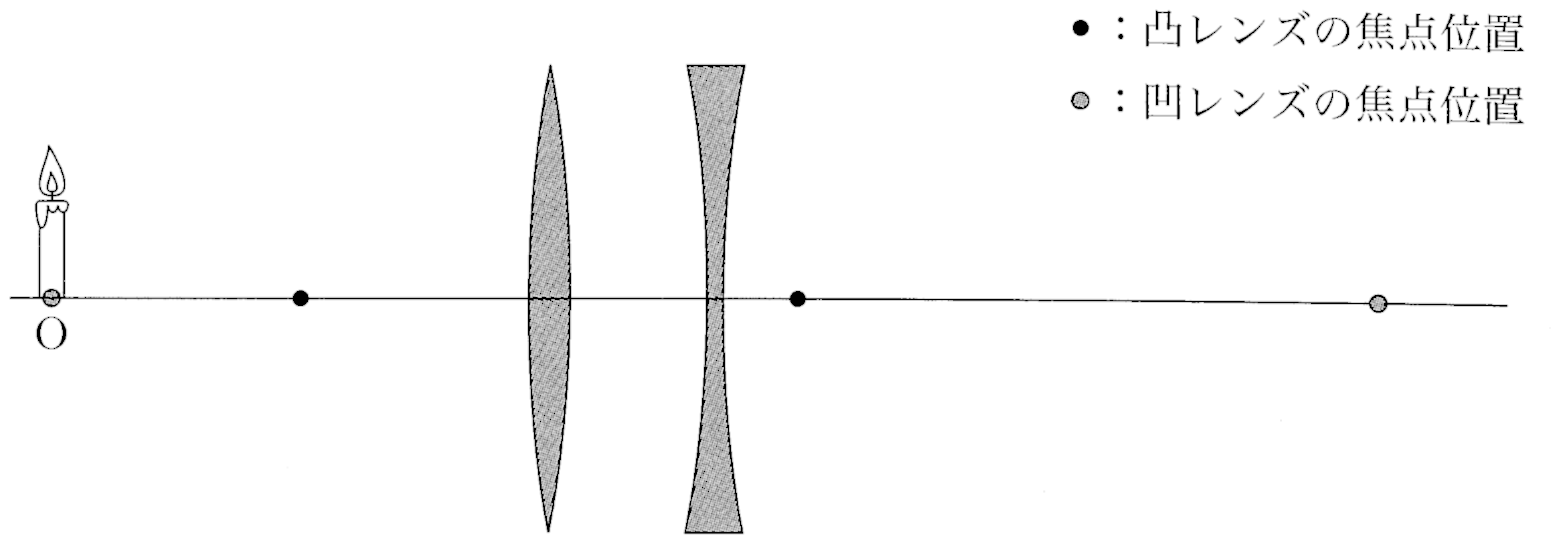
\includegraphics[keepaspectratio,width=110mm]{fig/n20_p67_zu.png}
\end{center}

\Mon{密着させた複合レンズによる像の作図}

\begin{zuright}{62mm}
\hspace{1zw}焦点距離が等しいレンズ2枚をぴったり隣り合わせにして，図の位置に光源を置いたとき，像の出来る位置を作図せよ．ただし，図中の点は，2枚のレンズから焦点距離分だけ離れた位置を表しており，2枚のレンズは十分に薄いものとする．
\zusep
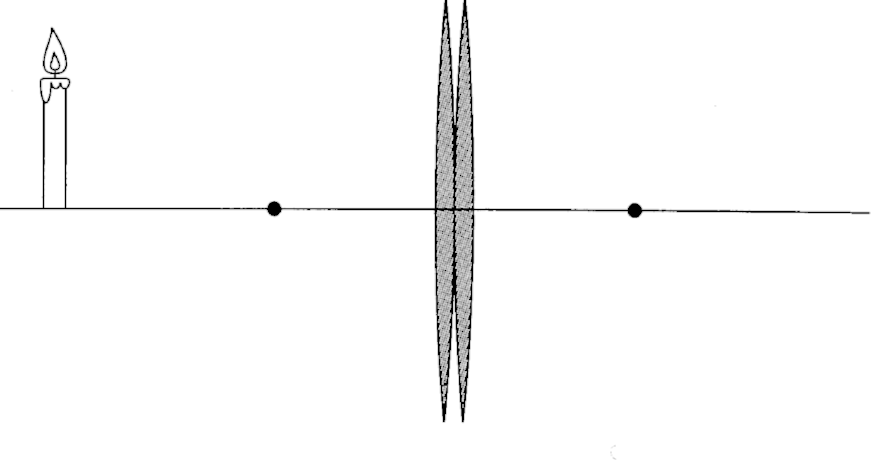
\includegraphics[keepaspectratio,width=62mm]{fig/n20_p68_zu.png}
\end{zuright}

\Mon{レンズと鏡による像}

% 原本は「図中の点は，各鏡から焦点距離分離れた位置を表している」だが，図の点は
% 凸レンズの焦点なので「レンズから」に直した（2026-09-10）。
\begin{zuright}{66mm}
\hspace{1zw}光源，凸レンズ，平面鏡が図のように置かれている．光源から出て，凸レンズを通り，平面鏡で反射され再び凸レンズを通った光が像を結ぶ位置を作図せよ．ただし，図中の点は，レンズから焦点距離分離れた位置を表している．
\zusep
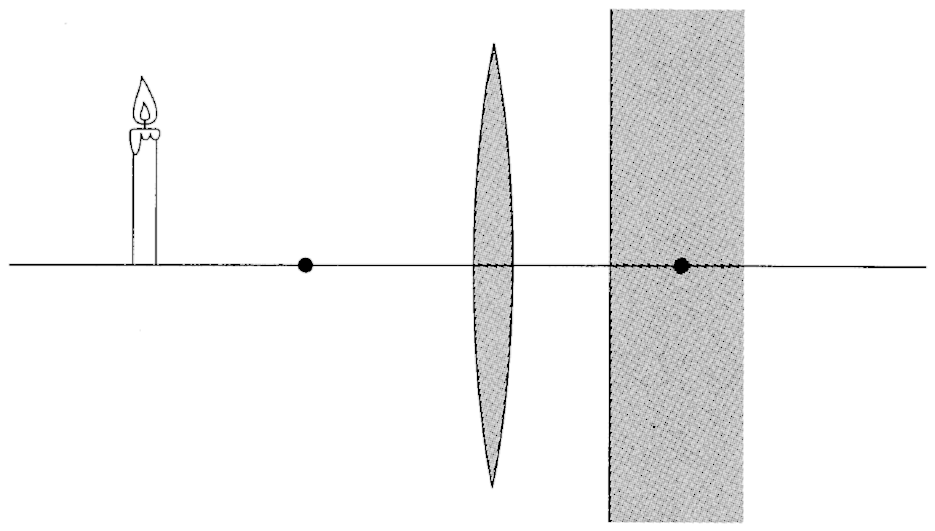
\includegraphics[keepaspectratio,width=66mm]{fig/n20_p69_zu.png}
\end{zuright}

\Mon{凸レンズ・凹レンズ}

\hspace{1zw}凸レンズもしくは凹レンズのいずれかを用いて像を観察した．以下の設問に答えよ．
\begin{komon}
\ko{1} レンズの手前側$10\U{cm}$のところに光源を置くと，3倍の大きさの実像が生じた．このレンズの種類は何か．また焦点距離は何$\U{cm}$か．
\ko{2} レンズの手前側$10\U{cm}$のところに光源を置くと，$\dfrac{1}{3}$倍の大きさの虚像が生じた．このレンズの種類は何か．また焦点距離は何$\U{cm}$か．
\end{komon}

\Mon[\Sitei]{像の移動速度}

% 原本の図には「2.0[cm]」と書かれているが，問題文の 2.0[m] と食い違う（誤植）。
% 図を TikZ で描き直して 2.0[m] に直した（texify_draft/mkfig_new20ans.py）。
\begin{zuright}{72mm}
\hspace{1zw}焦点距離$1.2\U{m}$の凸レンズの光軸上で，レンズの左側の$2.0\U{m}$の位置に光源$\mathrm{S}$がある．光源の大きさはレンズの焦点距離に比べて十分小さいものとして，以下の設問に答えよ．
\begin{komon}
\ko{1} レンズから像までの距離はいくらか．
\end{komon}
\zusep
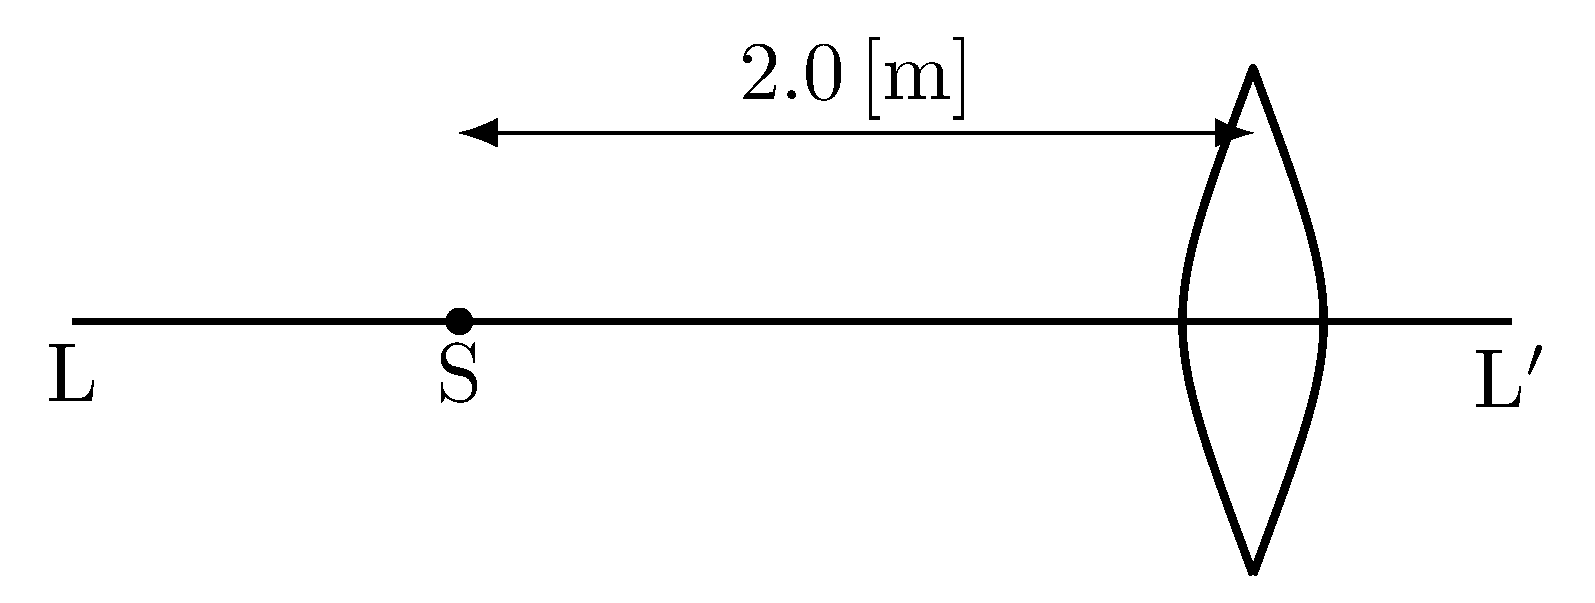
\includegraphics[keepaspectratio,width=72mm]{fig/n20_p71_zu.png}
\end{zuright}
\begin{komon}
\ko{2} この光源が，光軸$\mathrm{LL^\prime}$と垂直に，上方へ$0.4\U{m/s}$の速さで動き出したとすれば，像はどの方向にどれだけの速さで動き出すか．
\ko{3} 光源が静止していて，レンズが光軸$\mathrm{LL^\prime}$と垂直に上方へ$0.4\U{m/s}$の速さで動き出したとすれば，像はどの方向にどれだけの速さで動き出すか．
\end{komon}

\Mon{像の明るさ}

% 原本の設問(2)は「レンズとスクリーンの間の距離の条件」だが，解答は光源とスクリーンの
% 間の距離 a+b について答えている。設問側の誤植と判断して「光源とスクリーンの間の距離」
% に直した（2026-09-10）。
\hspace{1zw}薄い凸レンズの手前側$30\U{cm}$の光軸上にろうそくを置いたところ，レンズから$20\U{cm}$離れた向こう側のスクリーン上に実像を生じた．以下の設問に答えよ．
\begin{komon}
\ko{1} レンズに黒い紙をあてて上半分を覆った．このとき，像の位置，大きさ，明るさに変化が起こるか．起こるか否かを理由を付して答え，また変化する場合には，何がどのように変化するかを答えよ．
\ko{2} 光源とスクリーンの位置を固定し，その間にあるレンズを適当に動かすことでスクリーンに実像を結ばせたい．そのようなことが可能になるための光源とスクリーンの間の距離の条件を求めよ．
\end{komon}

\Mon{虫めがね}

\begin{zuright}{84mm}
\hspace{1zw}物体または像が目に対して張る角を{\gtfamily 視角}といい，視角が大きいほど物体や像が大きく見える．虫めがねの倍率$M$は，図のように虫めがねを使用せずに物体を明視距離$D\U{m}$（人間の目が最も疲れずに物体を見ることの出来る距離）に置いて見たときの視角を$\theta$，虫めがねによる像を明視距離$D\U{m}$に作ってこれを見たときの視角を$\theta^\prime$とするとき，$M=\dfrac{\theta^\prime}{\theta}$で表される．
\zusep
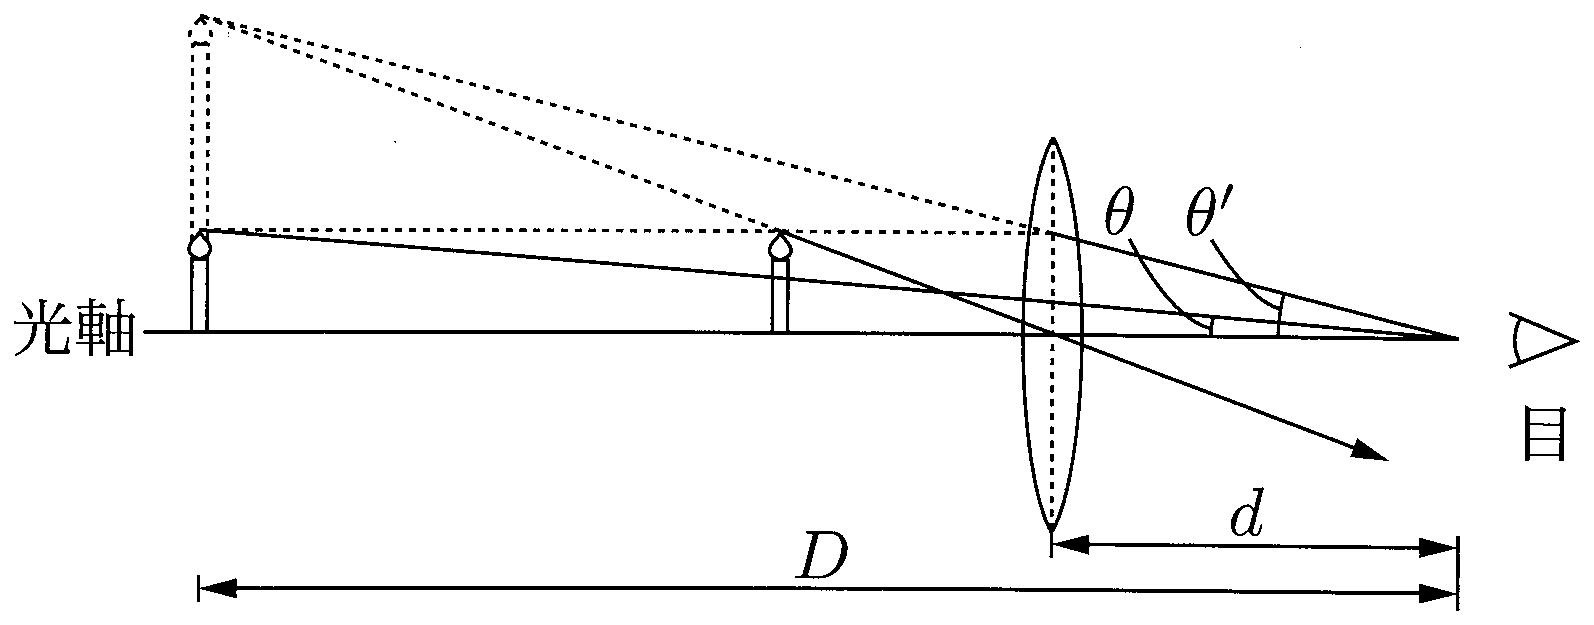
\includegraphics[keepaspectratio,width=84mm]{fig/n20_p73_zu.png}
\end{zuright}

\hspace{1zw}焦点距離$f\U{m}$の虫めがねを目から$d\U{m}$だけ離して用いて見る場合について，以下の設問に答えよ．
\begin{komon}
\ko{1} 虫めがねによる像を目から明視距離$D\U{m}$の位置に作るには，物体をレンズからどれだけ離せばよいか．
\ko{2} $\theta$, $\theta^\prime\ll 1$として一次近似$\tan\theta\fallingdotseq\theta$, $\tan\theta^\prime\fallingdotseq\theta^\prime$を利用して，このときの倍率を$f$, $D$, $d$で表せ．
\end{komon}

\Mon[\Sitei]{複合レンズ}

\begin{zuright}{76mm}
\hspace{1zw}平面鏡$\mathrm{D}$に垂直な直線上に，点光源$\mathrm{A}$，焦点距離$20\U{cm}$の凸レンズ$\mathrm{B}$，焦点距離$30\U{cm}$の凹レンズ$\mathrm{C}$を置く．$\mathrm{AD}$間の距離を$85\U{cm}$，$\mathrm{BD}$間の距離を$45\U{cm}$とするとき，点光源を出た光が平面鏡で反射し，再び$\mathrm{A}$点で像を結ぶためには，$\mathrm{DC}$間の距離をいくらにすればよいか．
\zusep
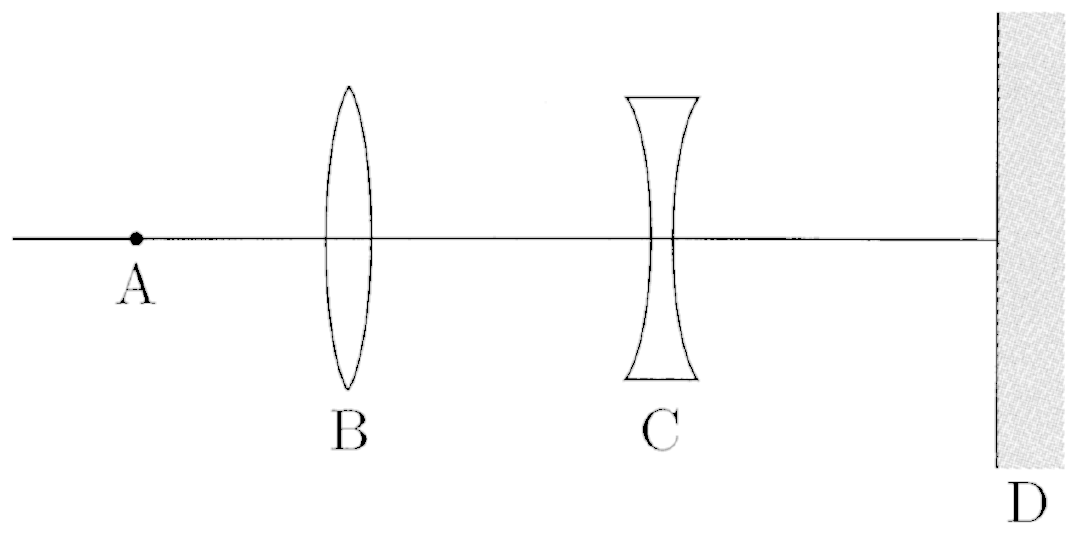
\includegraphics[keepaspectratio,width=76mm]{fig/n20_p74_zu.png}
\end{zuright}

\filbreak
\Rank{C問題}

\Mon{顕微鏡}

% 原本は「明視距離 D[m]」だが，f1・f2・a・d はすべて [cm] で，解答の式
% |CC'/AA'| = (D/f2)(f1/(a-f1)) も同じ単位でなければ成立しない。[cm] に直した。
\begin{zuright}{54mm}
\hspace{1zw}2枚の凸レンズを組み合わせて顕微鏡を作ることを考える．対物レンズ$\mathrm{L_1}$の焦点距離は$f_1\U{cm}$，接眼レンズ$\mathrm{L_2}$の焦点距離は$f_2\U{cm}$である．物体$\mathrm{AA^\prime}$を対物レンズ$\mathrm{L_1}$から距離$a\U{cm}$（$>f_1$）の位置におく．二つのレンズの距離を調節し，接眼レンズ$\mathrm{L_2}$から距離$f_2\U{cm}$だけ離れた位置から観察し，$\mathrm{L_2}$によって明視距離$D\U{cm}$の位置に虚像$\mathrm{CC^\prime}$を作ってこれを観察するのが顕微鏡である．これについて，以下の設問に答えよ．
\begin{komon}
\ko{1} $\mathrm{L_1}$によってできる実像$\mathrm{BB^\prime}$は$\mathrm{L_1}$からどれだけ上方の位置に出来るか．
\ko{2} 二つのレンズの焦点間の距離$d\U{cm}$をどのような範囲の値にすれば，レンズ$\mathrm{L_2}$によって作られる$\mathrm{BB^\prime}$の虚像が見えるか（右図の$\mathrm{BB^\prime}$は必ずしもこの位置とは限らない）．
\ko{3} 虚像が明視位置に出来るという条件を考えることにより，顕微鏡の倍率$\left|\dfrac{\mathrm{CC^\prime}}{\mathrm{AA^\prime}}\right|$を$a$, $D$, $f_1$, $f_2$を用いて表せ．
\end{komon}
\zusep
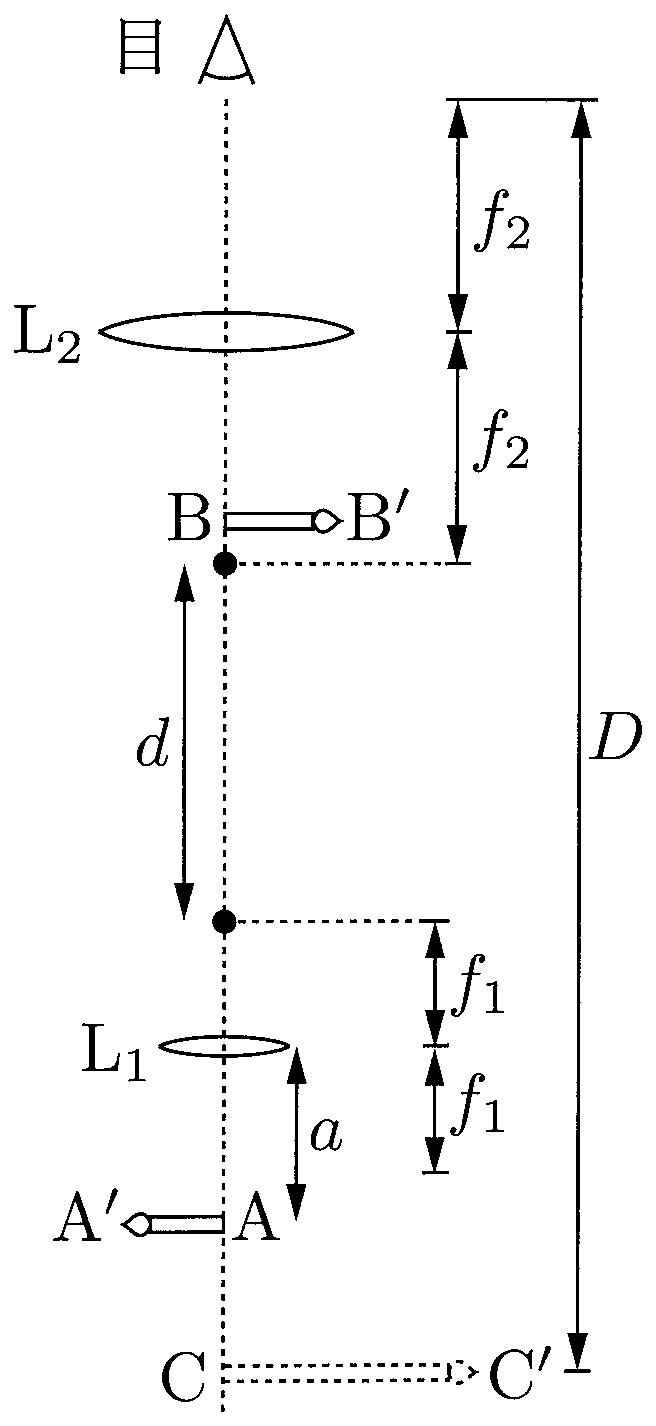
\includegraphics[keepaspectratio,width=54mm]{fig/n20_p75_zu.png}
\end{zuright}

\newpage

\KaiTitle{第20回　レンズと球面鏡}
\setlength{\columnseprule}{0.4pt}
\begin{multicols}{2}
\raggedcolumns

\Rank{A問題}
\MonN{63}{光の現象}\par\nopagebreak
\begin{sisin}
ここに挙げられているのは，日常生活で見られる光の現象である．知らないものも含まれていたと思うが，この機会に覚えておこう．
\end{sisin}
\KaiHead
\begin{komon}
\ko{1} \MARU{3}\ {\gtfamily 偏光}\Ans

       サングラスには偏光レンズ（特定の振動方向の光のみを通すようなレンズ）がついている．ガラスの表面で光が反射すると偏光が起こるため，反射光は特定の振動方向に偏る．したがって偏光レンズを用いて反射光を取り除けば，ショーウィンドウの中からの光がよく見えることになる．
\ko{2} \MARU{2}\ {\gtfamily 回折格子}\Ans

       コンパクトディスクの表面には，大小の凹凸が同心円状に並んでいるため，回折格子のように非常に細い溝をつけたものと同じ働きをする．反射光の強め合う方向は光の波長によって異なるので，白色光（可視領域のあらゆる波長の光を含む光線）を当てるとコンパクトディスクは美しく色づいて見える．詳しくは第19回の練習［62］で扱った．
\ko{3} \MARU{4}\ {\gtfamily 散乱}\Ans

       光の散乱とは，光が微粒子に当たると進行方向以外に散っていく現象のことを言い，一般に波長の短い光ほど散乱されやすい．また，赤い光は可視光の中でも波長が長い．地平線近くにある朝日や夕日から出た光は日中に比べて大気中を通過する距離が長くなるため，散乱されにくい赤色の光をより多く含むようになり，赤く見える．
\ko{4} \MARU{1}\ {\gtfamily 分散}\Ans

       屈折率は光の波長によって異なるため，白色光（あらゆる波長の光を含む光のこと）が物質に入射すると，光は波長ごとに分離して屈折していく．この現象を光の分散という．屈折率の大きい物質ほど分散の程度が大きい．ダイヤモンドの屈折率はガラスなどに比べるとかなり大きい（ガラスの屈折率が約1.5であるのに対してダイヤモンドの屈折率は約2.4）ので分散の程度が大きく，光が波長ごとに分かれていくので美しく色づいて見える．
\end{komon}

\Rank{B問題}
\MonN[\Sitei]{64}{レンズによる像の作図}\par\nopagebreak
% 原本の（指針）は凸レンズについても「手前側の焦点から直進したかのように進む光」と
% 書いているが，これは凹レンズの記述をそのまま写した誤りなので「向こう側の焦点を
% 通る光」に直した（2026-09-10）。
\begin{sisin}
凸レンズの場合，{\gtfamily \MARU{1}光軸に平行に出て向こう側の焦点を通る光}，{\gtfamily \MARU{2}レンズの中心$\mathrm{O}$を通過してそのまま直進する光}を，凹レンズの場合，{\gtfamily \MARU{1}光軸に平行に出て手前側の焦点から直進したかのように進む光}，{\gtfamily \MARU{2}レンズの中心$\mathrm{O}$を通過してそのまま直進する光}を書き込んで交点を求めると描きやすいことが多い．

虚光源の扱いについては，扱いに注意して欲しい．虚光源の位置から光が出ているのではなく，{\gtfamily その位置に向かって光が集まってきている}様に，入射光を考えなくてはいけない．
\end{sisin}
\KaiHead
\hspace{1zw}光軸に平行に入射する光と，レンズの中心を直進する光により，像の位置は次のように作図される．
\begin{center}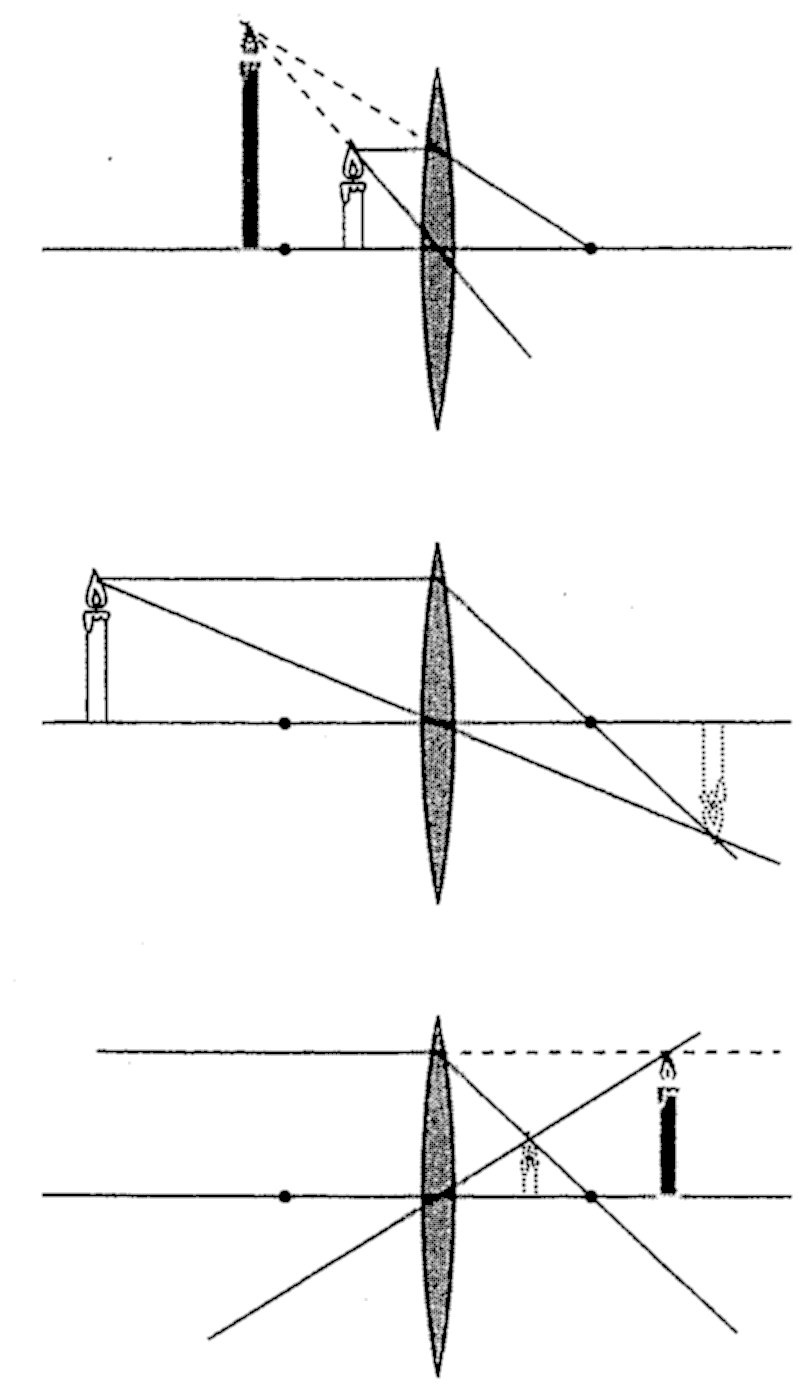
\includegraphics[keepaspectratio,width=62mm]{fig/n20_a64_conv.png}\end{center}
\begin{center}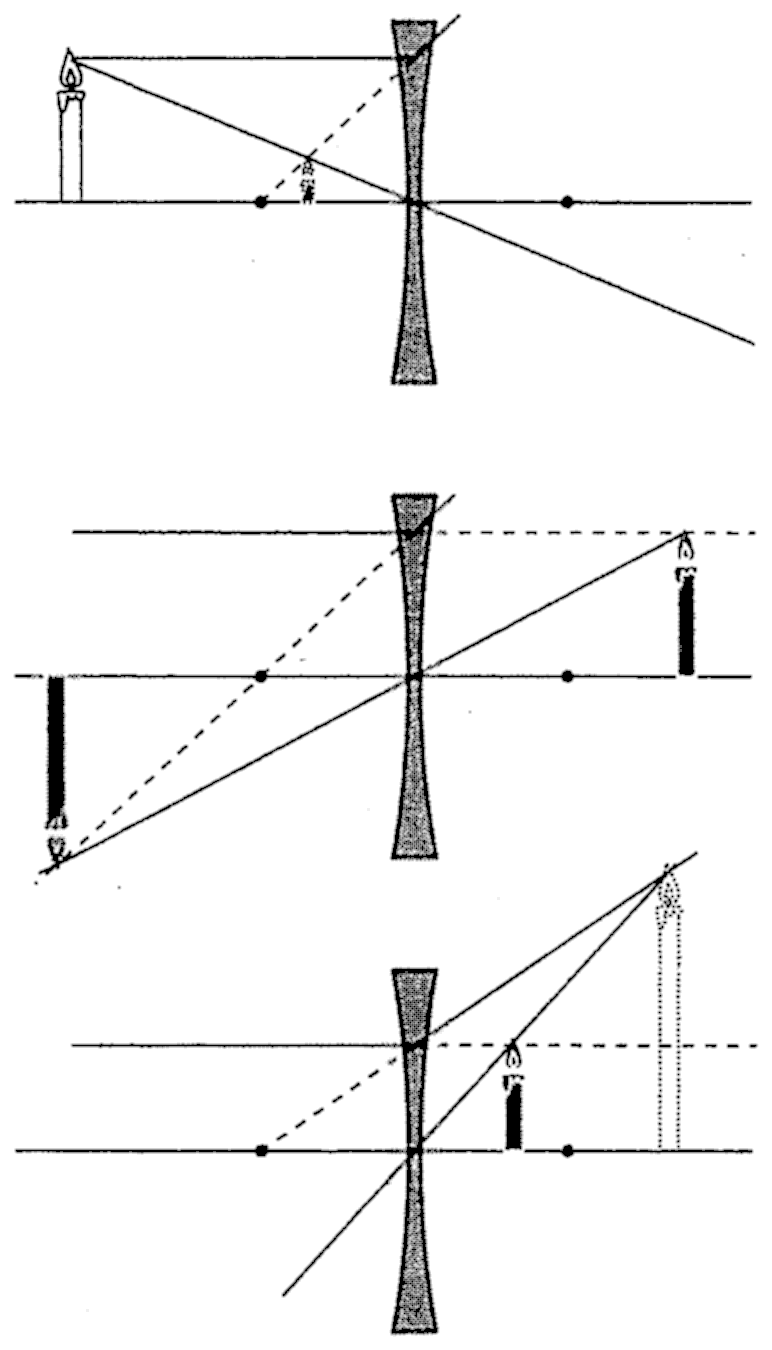
\includegraphics[keepaspectratio,width=62mm]{fig/n20_a64_conc.png}\end{center}
\hspace{1zw}各像の種類は，順に\\
\hspace*{1zw}凸レンズ：正立虚像，倒立実像，正立実像\\
\hspace*{1zw}凹レンズ：正立虚像，倒立虚像，正立実像\\
となる．\hspace{0.25zw}\mbox{$\cdots$(答)}

\MonN{65}{鏡による像の作図}\par\nopagebreak
\begin{sisin}
レンズによる像と同様，{\gtfamily \MARU{1}鏡に光軸と平行に入射する光}，{\gtfamily \MARU{2}鏡の中央に入射する光}の反射光を元に作図するとよい．\MARU{1}については，凹面鏡の場合は手前側の，凸面鏡の場合は奥側の焦点を通る直線となるように反射される．\MARU{2}については，入射角と反射角が等しくなるよう，平面鏡によって反射された場合と同じように反射される．

なお，図には鏡の両側に点が打たれているが，{\gtfamily 焦点として働くのは，凹面鏡では手前側（光の来る側），凸面鏡では奥側の点}だけである．

結果的に，{\gtfamily 凹面鏡は凸レンズによる結像を，凸面鏡は凹レンズによる結像を，それぞれ反射面（レンズの位置）に関して折り返したもの}と同じになる．前問のレンズによる像と対応するよう，この問題は作られているので，是非見比べておいてほしい．
\end{sisin}
\KaiHead
\hspace{1zw}光軸に平行に入射する光と，鏡の中心で反射される光により，像の位置は次のように作図される．
\begin{center}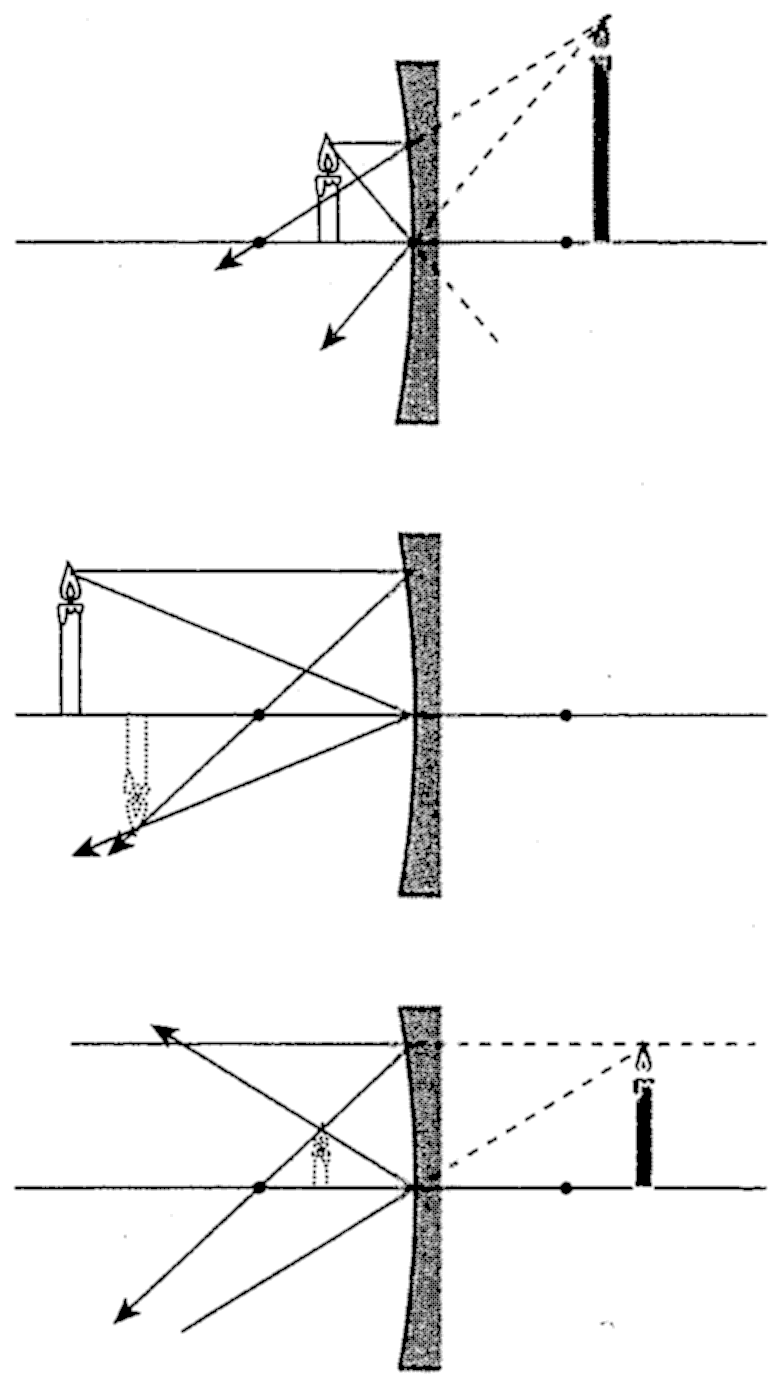
\includegraphics[keepaspectratio,width=62mm]{fig/n20_a65_conc.png}\end{center}
\begin{center}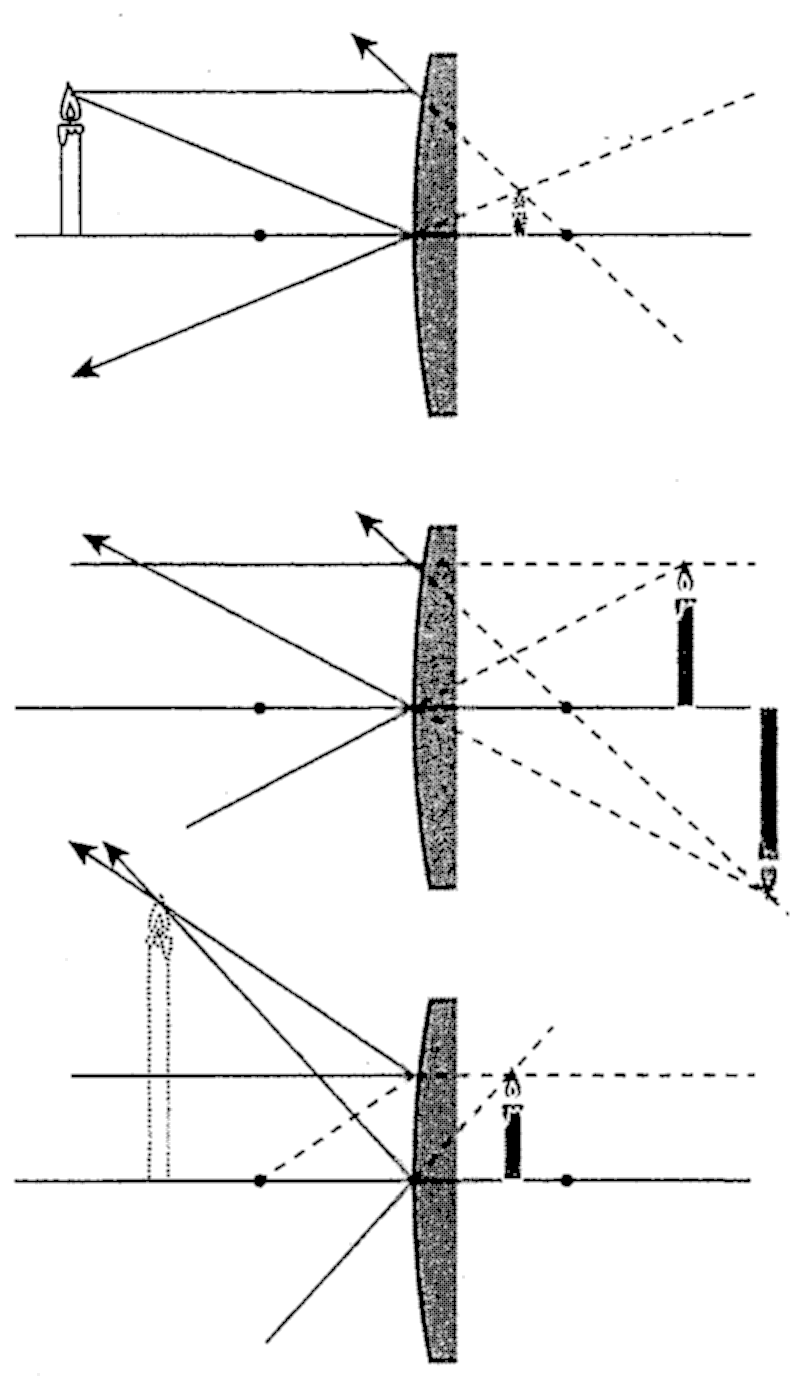
\includegraphics[keepaspectratio,width=62mm]{fig/n20_a65_conv.png}\end{center}
% 原本の解答は「凸レンズ：…／凹レンズ：…」と，前問の文をそのまま写した誤りなので
% 凹面鏡／凸面鏡に直した（2026-09-10）。
\hspace{1zw}各像の種類は，順に\\
\hspace*{1zw}凹面鏡：正立虚像，倒立実像，正立実像\\
\hspace*{1zw}凸面鏡：正立虚像，倒立虚像，正立実像\\
となる．\hspace{0.25zw}\mbox{$\cdots$(答)}

\MonN[\Sitei]{66}{近軸近似}\par\nopagebreak
\begin{sisin}
レンズは球面に近い曲面で構成されている．平行光が一点に集光する仕組みを証明する問題である．レンズと空気の界面での屈折の法則より，角度間の関係式を立てて，幾何的に考察をしていこう．
\end{sisin}
\KaiHead
\begin{komon}
% 原本は「右側の球面での反射を考えると」だが屈折の誤りなので直した（2026-09-10）。
% 加筆（2026-09-20）：なぜ入射角が $\theta$，屈折角が $\theta+\varphi$ になるのかが
% 書かれておらず（原本の図にも法線のラベルが無かった）図だけでは追えなかったので，
% 理由を明記し，図もラベル付きで描き直した（mkfig_new20ans.py の a66()）。
\ko{1} 左側の界面は平面なので，屈折による角度の変化はない．右側の球面で屈折するときの{\gtfamily 法線は，球の中心$\mathrm{O}$と入射点$\mathrm{A}$を結ぶ直線$\mathrm{OA}$}である．入射光は光軸に平行だから，入射光と$\mathrm{OA}$のなす角（入射角）は錯角により$\angle\mathrm{AOB}=\theta$に等しい．また，$\triangle\mathrm{AOP}$において$\mathrm{A}$における外角を考えると，屈折光と$\mathrm{OA}$のなす角（屈折角）は$\theta+\varphi$である．点$\mathrm{A}$のまわりを拡大すると次図のようになる．
       \begin{center}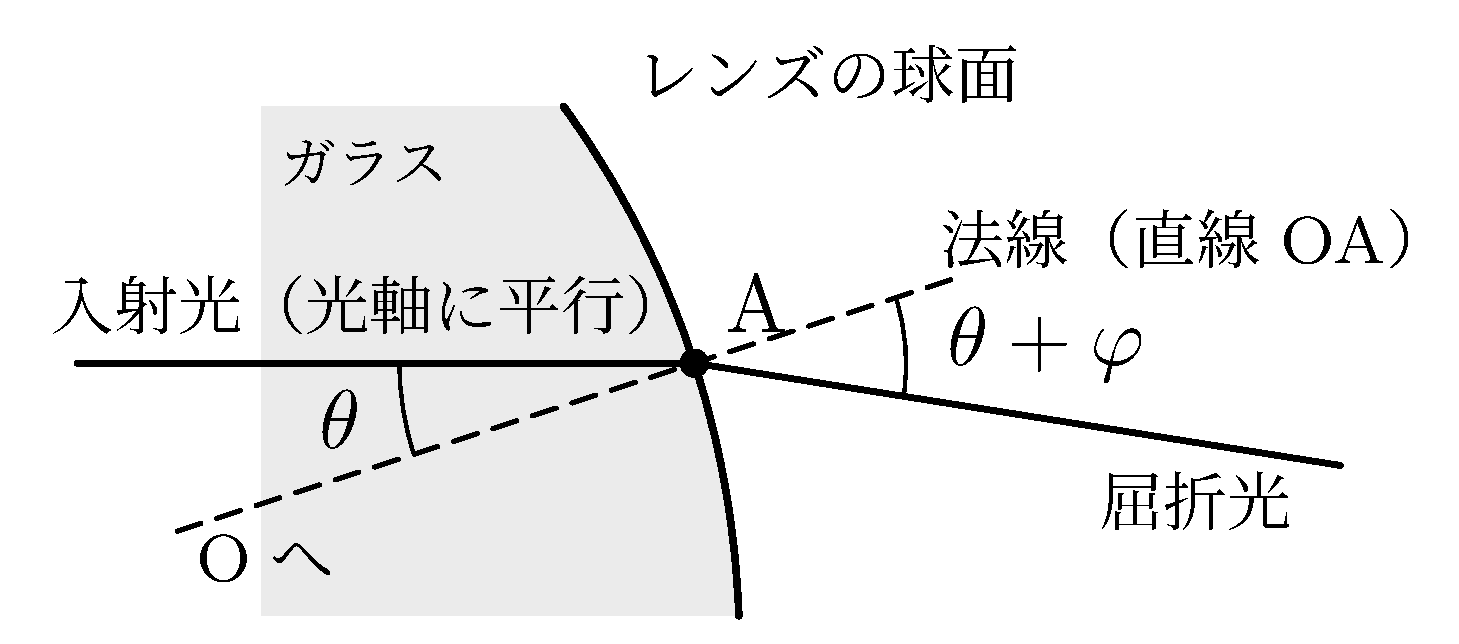
\includegraphics[keepaspectratio,width=68mm]{fig/n20_a66_zu.png}\end{center}
       よって屈折の法則より，
       \[n\sin\theta=\sin(\theta+\varphi)\Ans\]
\ko{2} $\theta$, $\varphi$は微小なので，(1)の式を近似して，
       \[n\theta=\theta+\varphi\ \Longleftrightarrow\ \varphi=(n-1)\theta\]
       図より，$\sin\theta=\dfrac{z}{R}$が成立する点に注意して，$\mathrm{BP}$間の距離は，
       \[\begin{aligned}\frac{z}{\tan\varphi}&\fallingdotseq\frac{z}{\varphi}=\frac{z}{(n-1)\theta}\\
         &\fallingdotseq\frac{z}{(n-1)\sin\theta}=\frac{R}{n-1}\end{aligned}\]
       この値は$z$に依らず一定となるので，焦点距離は
       \[\frac{R}{n-1}\Ans\]
\end{komon}

\MonN{67}{離れた複合レンズによる像の作図}\par\nopagebreak
\begin{sisin}
凸レンズによって曲げられた光は，凹レンズに入射する光と一致することを考えれば，{\gtfamily 凸レンズによる像の位置は凹レンズにとっての光源の位置になる}．

従って，まずは凸レンズによる写像で像ができる位置を，作図により求める．この際，凹レンズによる影響は考えずに，凸レンズだけであった場合，どこに集光するのかを考える．

次に，凸レンズによる像の位置を光源と考えて，凹レンズの写像を考えればよい．凸レンズの作図に用いた線は気にせず，凹レンズにとっての光源の位置から像を作図していく．
\end{sisin}
\KaiHead
\hspace{1zw}まず，凹レンズがなかった場合の，凸レンズによる像の位置は，次のように作図される．
\begin{center}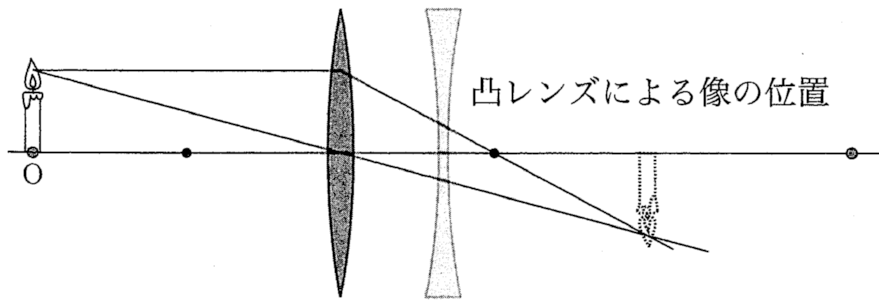
\includegraphics[keepaspectratio,width=72mm]{fig/n20_a67_zu1.png}\end{center}
\hspace{1zw}凹レンズは，この像の位置を光源（図より，虚光源となる）とした写像となるので，凹レンズによる像の位置は，次のようになる．
\begin{center}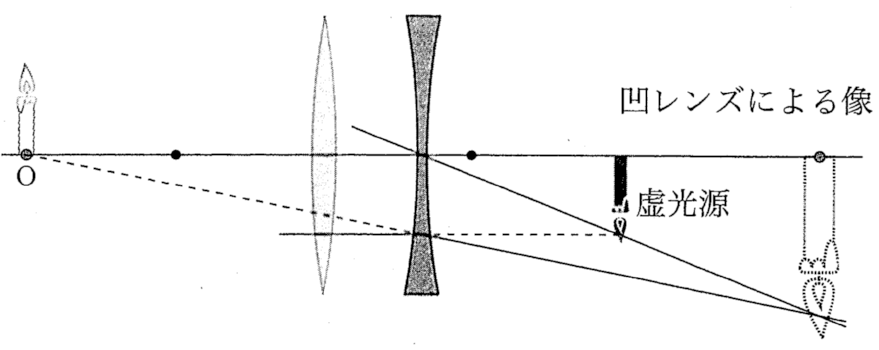
\includegraphics[keepaspectratio,width=72mm]{fig/n20_a67_zu2.png}\end{center}
\hspace{1zw}以上を合わせて，まとめて作図すると，次図のようになり，像は倒立実像ができる．
\begin{center}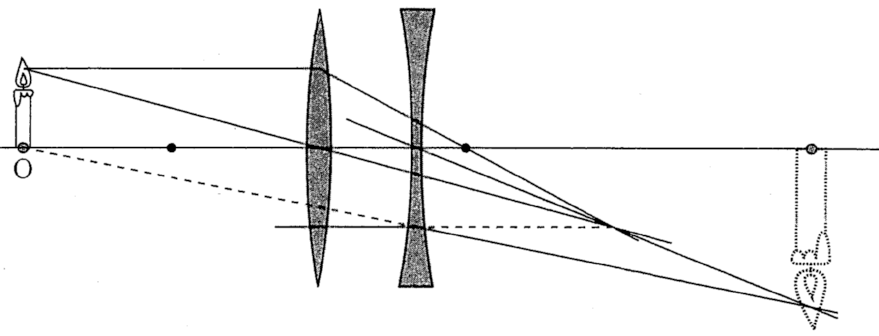
\includegraphics[keepaspectratio,width=72mm]{fig/n20_a67_zu3.png}\end{center}
\hspace*{\fill}\mbox{$\cdots$(答)}

\MonN{68}{密着させた複合レンズによる像の作図}\par\nopagebreak
\begin{sisin}
密着させた場合も，前問と同様，各レンズごとに作図すればよい．しかし，少し工夫をすると，作図を2回に分けずに終わらせることができる．

まず，密着しているので，レンズの中心は一致しているとみなせるため，合成レンズの中央に入射する光は直進するとしてよい．

もう一方の光については，光軸に平行に入射する光ではなく，{\gtfamily 手前側の焦点を通る光}について考えてみるとよい．手前側の焦点を通過して入射する光が1枚目の凸レンズを通ると，光軸に平行な光となるため，2枚目のレンズによる屈折で，奥側の焦点を通る光となる．

この2本の光の進み方は，1枚目のレンズによる像の位置を求めずに描けるため，手間が少なくて済む．
\end{sisin}
\KaiHead
\hspace{1zw}レンズに対し，\\
\hspace*{1zw}\MARU{1}\ レンズの中央に入射する光\\
\hspace*{1zw}\MARU{2}\ 手前の焦点を通過してレンズに入射する光\\
を考える．

\hspace{1zw}\MARU{1}については，十分に薄いレンズが密着しているので，どちらもレンズの中心を通るとみなしてよく，2枚のレンズを通過する前後で直進する．

\hspace{1zw}\MARU{2}については，1枚目のレンズにより，光軸と平行に進む光となるので，2枚目のレンズによる屈折では，奥側の焦点を通るように進む．

\hspace{1zw}以上2つの光の交点の位置を作図して，像の位置は次図のように求まる．
\begin{center}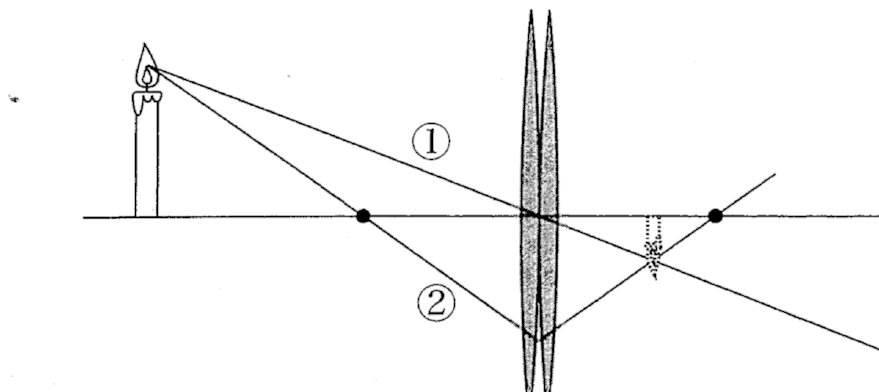
\includegraphics[keepaspectratio,width=62mm]{fig/n20_a68_zu.png}\end{center}
\hspace*{\fill}\mbox{$\cdots$(答)}

\MonN{69}{レンズと鏡による像}\par\nopagebreak
\begin{sisin}
合計3回分の写像を考えることになる．まずは凸レンズに左から右に入射する光による写像．その次に平面鏡による写像．最後に，凸レンズに右から左に入射する光による写像である．それぞれの場合で，像の位置がどこになるのかを丁寧に作図していく必要がある．
\end{sisin}
\KaiHead
\hspace{1zw}まず，光源から直接凸レンズに入射した光が，凸レンズによって像を結ぶ位置は次図のようになる．
\begin{center}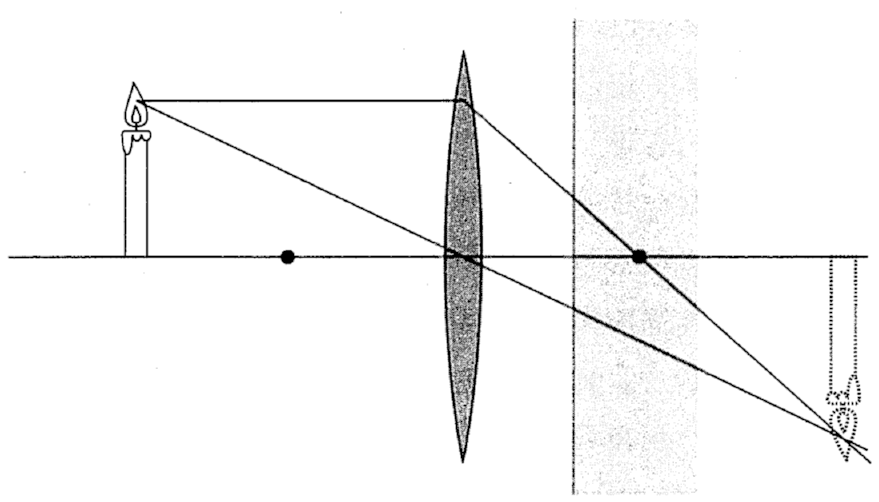
\includegraphics[keepaspectratio,width=62mm]{fig/n20_a69_zu1.png}\end{center}
\hspace{1zw}この像の位置は，平面鏡により，次図のように反射された位置に像を結ぶ．
\begin{center}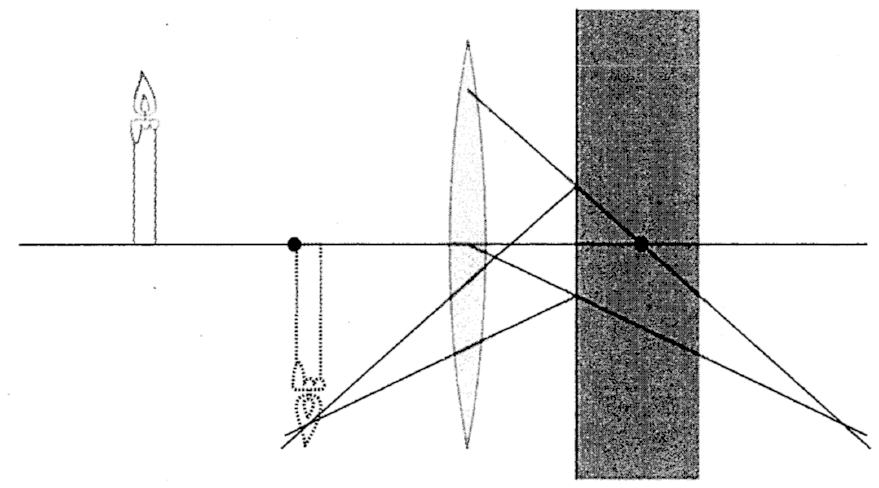
\includegraphics[keepaspectratio,width=62mm]{fig/n20_a69_zu2.png}\end{center}
\hspace{1zw}よって，この位置を光源（図より虚光源となる）とする凸レンズによる像の位置は，次図のように作図される．
\begin{center}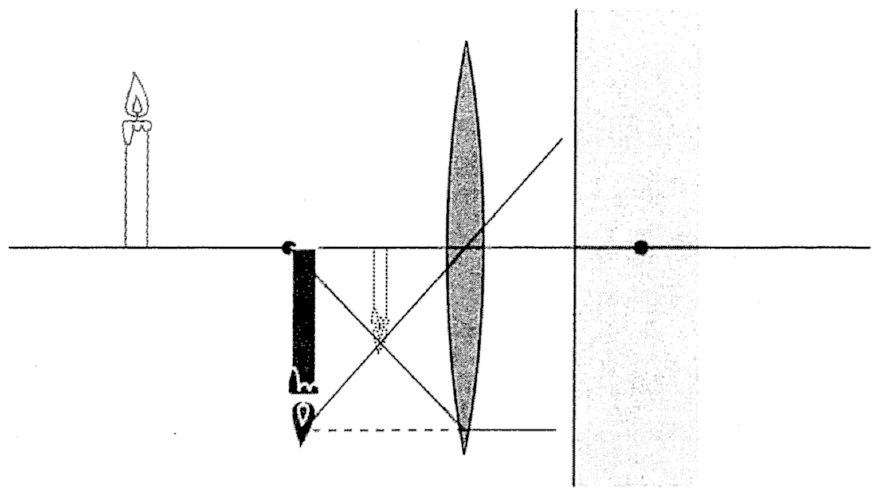
\includegraphics[keepaspectratio,width=62mm]{fig/n20_a69_zu3.png}\end{center}
\hspace{1zw}以上をまとめて，次図のように倒立実像ができる．
\begin{center}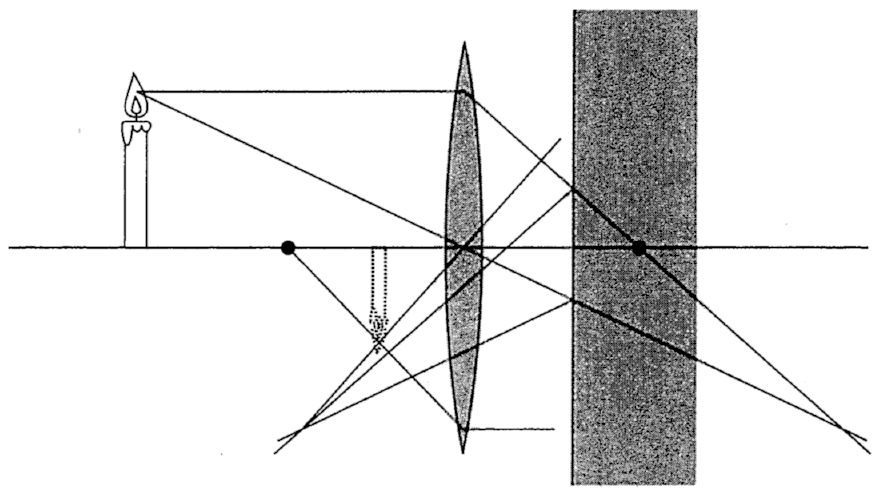
\includegraphics[keepaspectratio,width=62mm]{fig/n20_a69_zu4.png}\end{center}
\hspace*{\fill}\mbox{$\cdots$(答)}

\MonN{70}{凸レンズ・凹レンズ}\par\nopagebreak
\begin{sisin}
写像公式$\dfrac{1}{a}+\dfrac{1}{b}=\dfrac{1}{f}$および倍率公式$m=\left|\dfrac{b}{a}\right|$をうまく組み合わせて考えていく問題である．倍率公式だけでは像の位置$b$の正負が不明であるが，{\gtfamily 実像なら$b>0$，虚像なら$b<0$}であることから$b$の値を決定しよう．
\end{sisin}
\KaiHead
\hspace{1zw}写像公式$\dfrac{1}{a}+\dfrac{1}{b}=\dfrac{1}{f}$を利用して考える．
\begin{komon}
\ko{1} $a=+10\U{cm}$であり，倍率が3倍であるから
       \[3=\left|\frac{b}{+10}\right|\]
       ゆえ，$b=\pm 30\U{cm}$である．出来たのは実像であるから$b>0$である．よって，$b=+30\U{cm}$．

       これを写像公式に当てはめると，
       \[\frac{1}{10}+\frac{1}{30}=\frac{1}{f}\]
       であるから，これを解いて，
       \[f=\frac{30}{4}=+7.5\U{cm}\]
       である．$f>0$であるからレンズは凸レンズであり，その焦点距離は$7.5\U{cm}$である．\hspace{0.25zw}\mbox{$\cdots$(答)}
\ko{2} $a=+10\U{cm}$であり，倍率が$\dfrac{1}{3}$倍であるから
       \[\frac{1}{3}=\left|\frac{b}{+10}\right|\]
       ゆえ，$b=\pm\dfrac{10}{3}\U{cm}$である．出来たのは虚像であるから$b<0$である．よって，$b=-\dfrac{10}{3}\U{cm}$．

       これを写像公式に当てはめると，
       \[\frac{1}{10}-\frac{3}{10}=\frac{1}{f}\]
       であるから，これを解いて，
       \[f=-5.0\U{cm}\]
       である．$f<0$であるからレンズは凹レンズであり，その焦点距離は$5.0\U{cm}$である．\hspace{0.25zw}\mbox{$\cdots$(答)}
\end{komon}

\MonN[\Sitei]{71}{像の移動速度}\par\nopagebreak
\begin{sisin}
本問のような点光源の場合には，作図法による像の位置の把握，すなわち\MARU{1}光軸に平行に出て向こう側の焦点を通るような光，\MARU{2}レンズの中心$\mathrm{O}$を通過してそのまま直進する光，の二つを作図し，交点を求める，という考え方は利用できない（\MARU{1}の光が作図できないため）が，{\gtfamily 点光源の場合にも写像公式が成立し，点光源から出た光はこの式によって決まる像の位置に収束する}（このことは物体の大きさがどんどん小さくなっていって最終的に無限小になって点光源になったと考えれば明らかである）．

点光源が光軸から離れるように移動した場合，これは光軸上に大きさがある光源が乗っているのと同じパターンに帰着できるので，像がレンズからどれだけ離れているのかは写像公式を利用して，また光軸からどれだけ離れているかは倍率公式を利用すれば分かる．位置関係を把握する図を簡単に描いて考えよう．
\end{sisin}
\KaiHead
\begin{komon}
\ko{1} 写像公式を利用すると，
       \[\frac{1}{2.0}+\frac{1}{b}=\frac{1}{1.2}\]
       であるから，これを解いて，
       \[b=+3.0\U{m}\Ans\]
       である．すなわち，光源から出てレンズを通った光は，レンズの奥側$3.0\U{m}$の位置に収束する．
       \begin{center}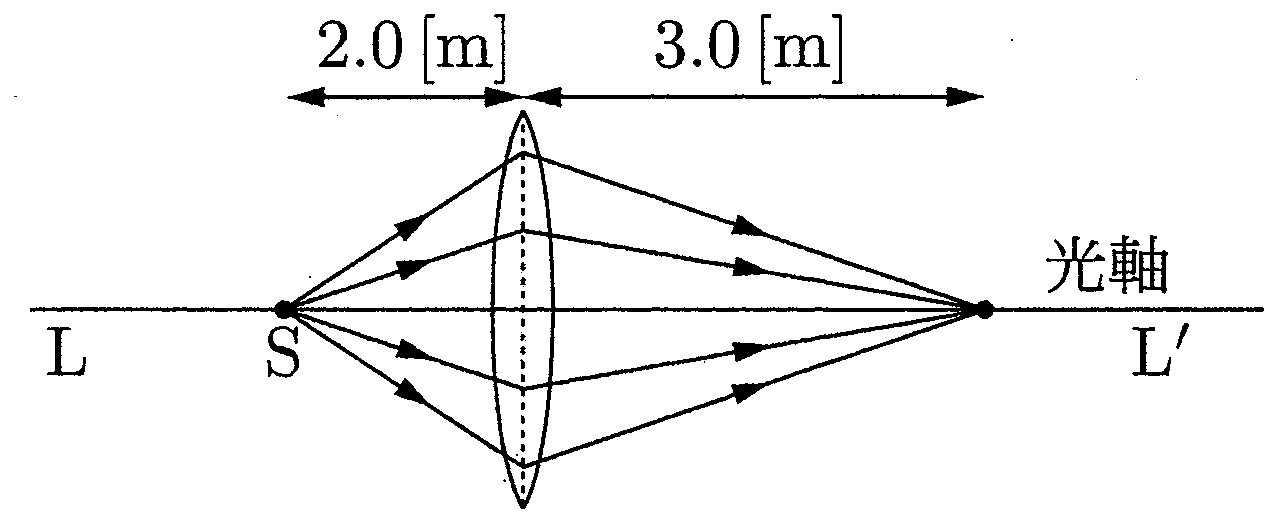
\includegraphics[keepaspectratio,width=62mm]{fig/n20_a71_zu1.png}\end{center}
\ko{2} 動き始めてから$t\U{s}$後には，光源は光軸から$0.4t\U{m}$だけ離れているが，レンズからの距離は変わっていないので像の出来る位置はやはりレンズの奥側$3.0\U{m}$の位置である．これを図示すると次図のようになる．
       \begin{center}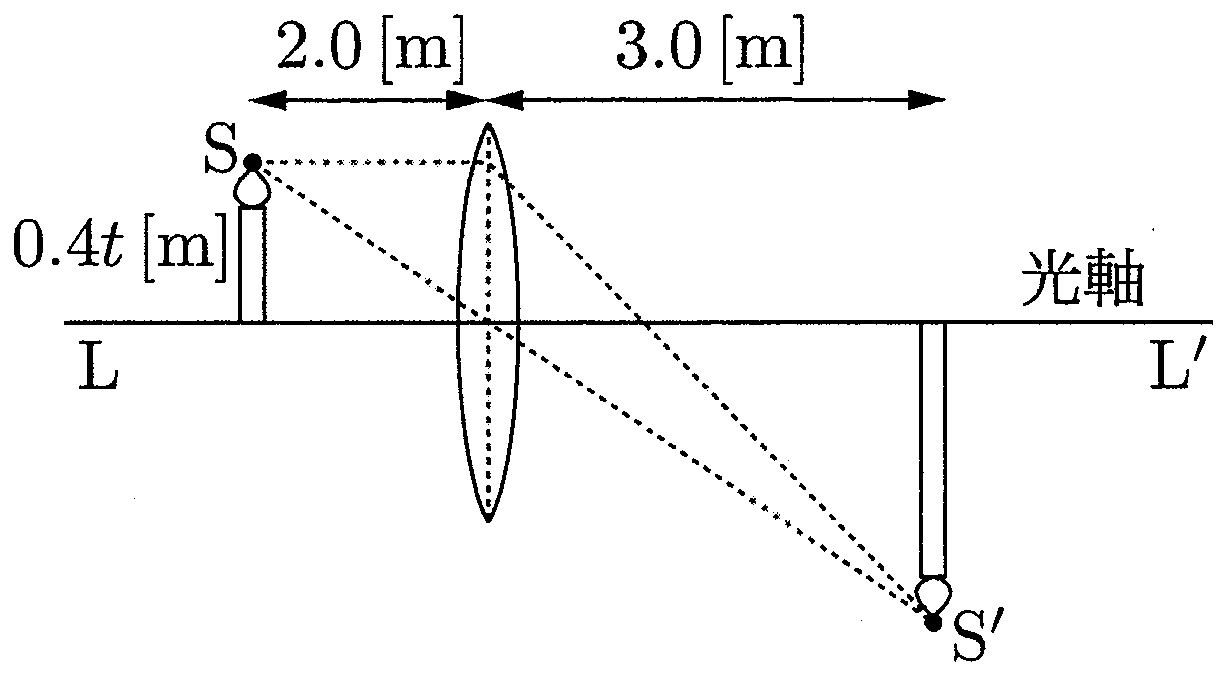
\includegraphics[keepaspectratio,width=62mm]{fig/n20_a71_zu2.png}\end{center}
       よって，このとき光源$\mathrm{S}$から出た光は上図の$\mathrm{S^\prime}$に収束する．このときの倍率は
       \[m=\left|\frac{3.0}{2.0}\right|=1.5\ \text{倍}\]
       であるから，$\mathrm{S^\prime}$は光軸から
       \[0.4t\times 1.5=0.6t\U{m}\]
       だけ離れている．よって，像$\mathrm{S^\prime}$は光軸から下方向へ等速度運動し，その移動する速さは
       \[\frac{d}{dt}(0.6t)=0.6\U{m/s}\Ans\]
\ko{3} 動き始めてから$t\U{s}$後には，レンズおよび光軸は元の位置から$0.4t\U{m}$だけ上へずれているが，レンズからの距離は変わっていないので像の出来る位置はやはりレンズの奥側$3.0\U{m}$の位置である．これを図示すると次図のようになる．
       \begin{center}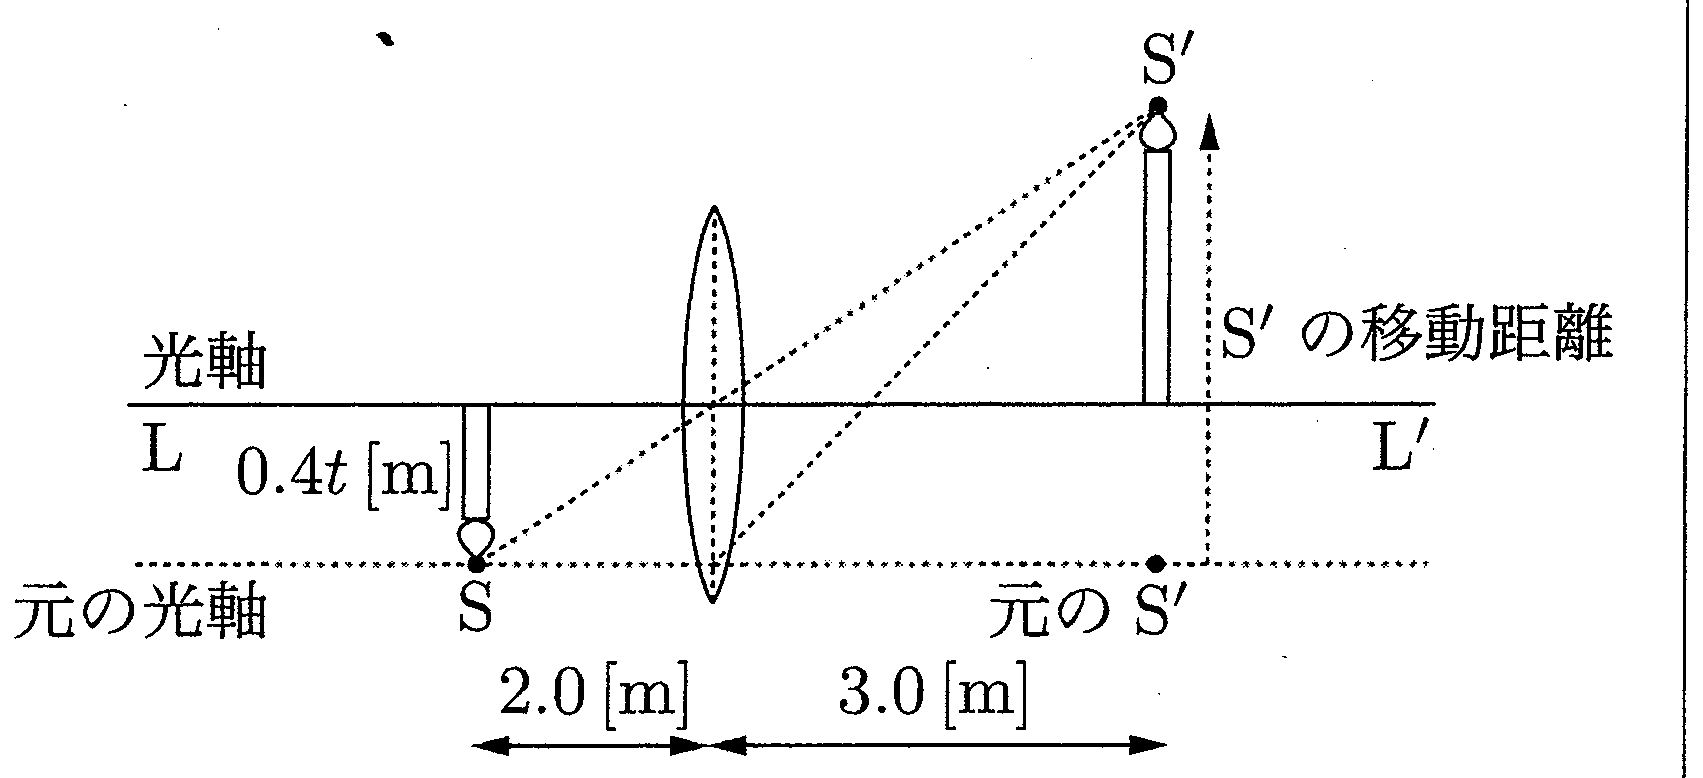
\includegraphics[keepaspectratio,width=68mm]{fig/n20_a71_zu3.png}\end{center}
       よって，このとき光源$\mathrm{S}$から出た光は上図の$\mathrm{S^\prime}$に収束する．このときの倍率も$1.5$倍であるから，$\mathrm{S^\prime}$は現在の光軸からは上方に
       \[0.4t\times 1.5=0.6t\U{m}\]
       だけ離れており，元の光軸からは上方に
       \[0.6t+0.4t=1.0t\U{m}\]
       だけ離れている．よって，像$\mathrm{S^\prime}$は元の位置から上方向へ等速度運動し，その移動する速さは
       \[\frac{d}{dt}(1.0t)=1.0\U{m/s}\Ans\]
\end{komon}

\MonN{72}{像の明るさ}\par\nopagebreak
\begin{sisin}
光源からは光はさまざまな方向に放出されており，像の位置には，光源から放出されてレンズを通るすべての光が収束している．よって，レンズの一部を隠した場合には，{\gtfamily 覆われていない部分を通った光しか像の位置に収束できない}．このことを図で考えて，像の位置，大きさ，明るさにどのような変化が起こるのかを考えよう．
\end{sisin}
\KaiHead
\begin{komon}
\ko{1} 光源からさまざまな方向へ出た光はレンズに対して入射したあと屈折を起こしてレンズの奥側の像の位置へと収束するように進む．特にろうそくの一番先端の部分に注目すると，ここから出た光は図のように進んで一点に集まる．
       \begin{center}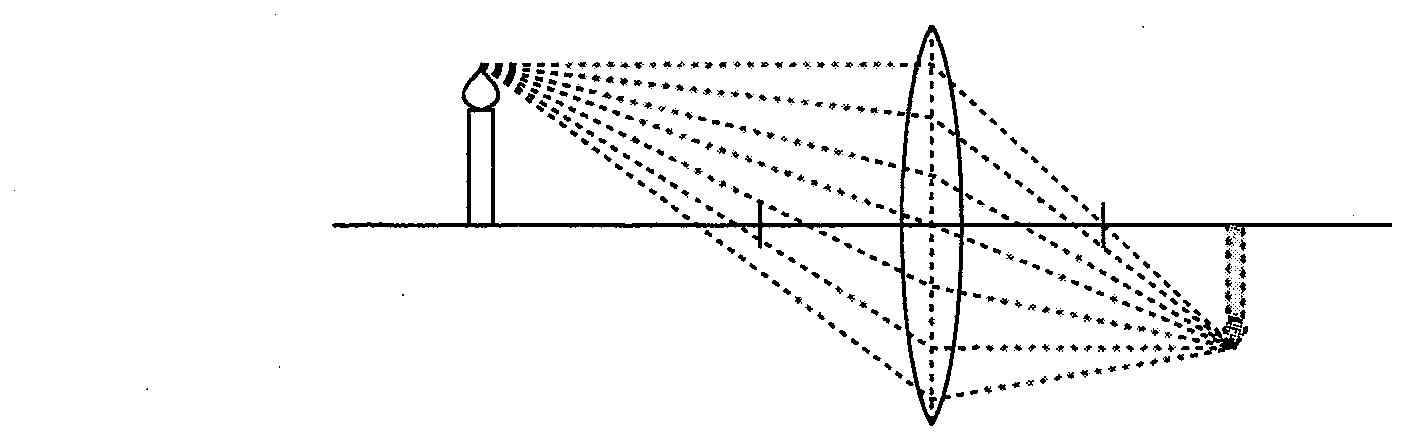
\includegraphics[keepaspectratio,width=62mm]{fig/n20_a72_zu1.png}\end{center}
       また，ろうそくのつけ根の部分から出た光については，レンズに入射したあと下の図のようにして屈折して，実像のつけ根へと収束する．
       \begin{center}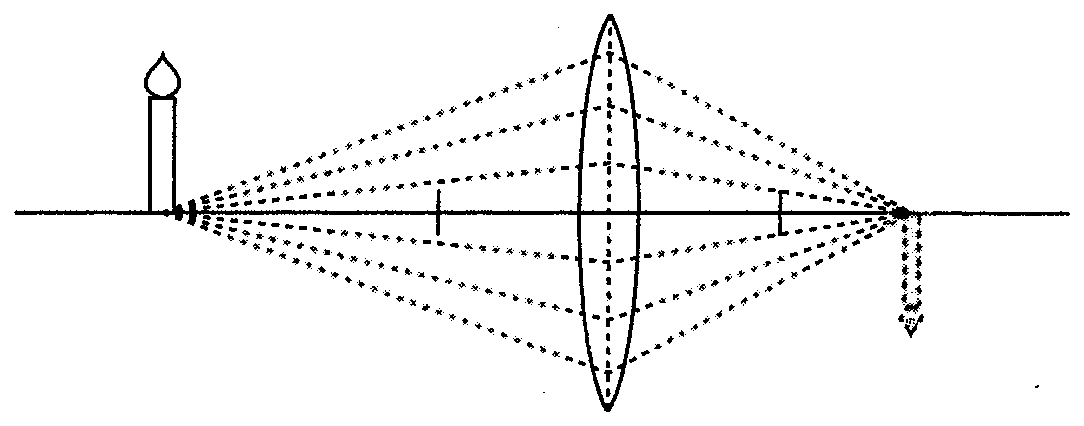
\includegraphics[keepaspectratio,width=62mm]{fig/n20_a72_zu2.png}\end{center}
       これらの二つの図においてレンズの上半分を覆うと，像の位置へはレンズ下半分を通過した光しか到達しなくなる．
       \begin{center}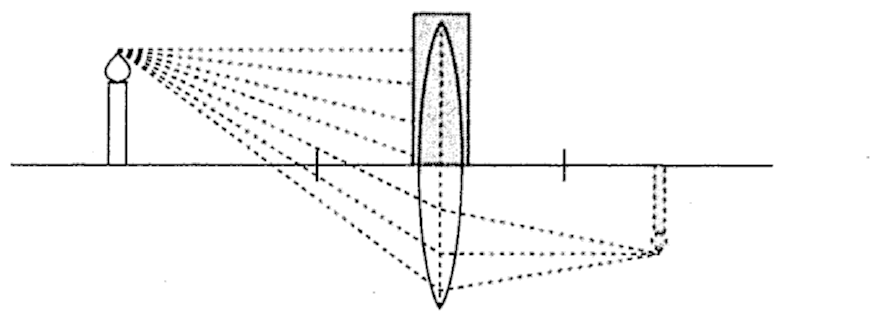
\includegraphics[keepaspectratio,width=62mm]{fig/n20_a72_zu3.png}\end{center}
       \begin{center}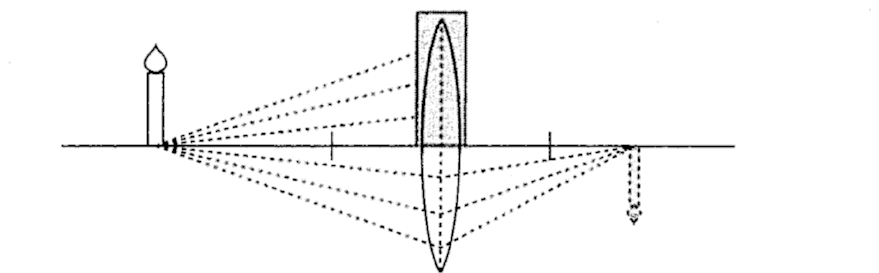
\includegraphics[keepaspectratio,width=62mm]{fig/n20_a72_zu4.png}\end{center}
       これらの図から分かるように，レンズの上半分を隠しても屈折光の収束する位置は変わらず，また実像が欠けることもないが，レンズを通過する光の量が約半分になるため，実像の明るさは半減する．よってまとめると，\\
       \hspace*{1zw}像の位置，大きさは不変．\\
       \hspace*{1zw}像の明るさはほぼ半減する．\hspace{0.25zw}\mbox{$\cdots$(答)}
\ko{2} まず，このレンズの焦点距離を求める．最初の状態に対して写像公式を適用すると，
       \[\frac{1}{30}+\frac{1}{20}=\frac{1}{f}\quad\text{より}\quad f=12\U{cm}\]
       である．

       レンズとスクリーンの位置を動かして，レンズと光源間の距離を$a\U{cm}$，スクリーンとレンズとの距離を$b\U{cm}$とすると，写像公式より
       \[\frac{1}{a}+\frac{1}{b}=\frac{1}{12}\]
       が成立するので，
       \[b=\left(\frac{1}{12}-\frac{1}{a}\right)^{-1}=\frac{12a}{a-12}\U{cm}\]
       である．凸レンズの場合の写像公式の直角双曲線のカーブを考えると，実像が出来る（すなわち$b>0$となる）ためには，
       \begin{center}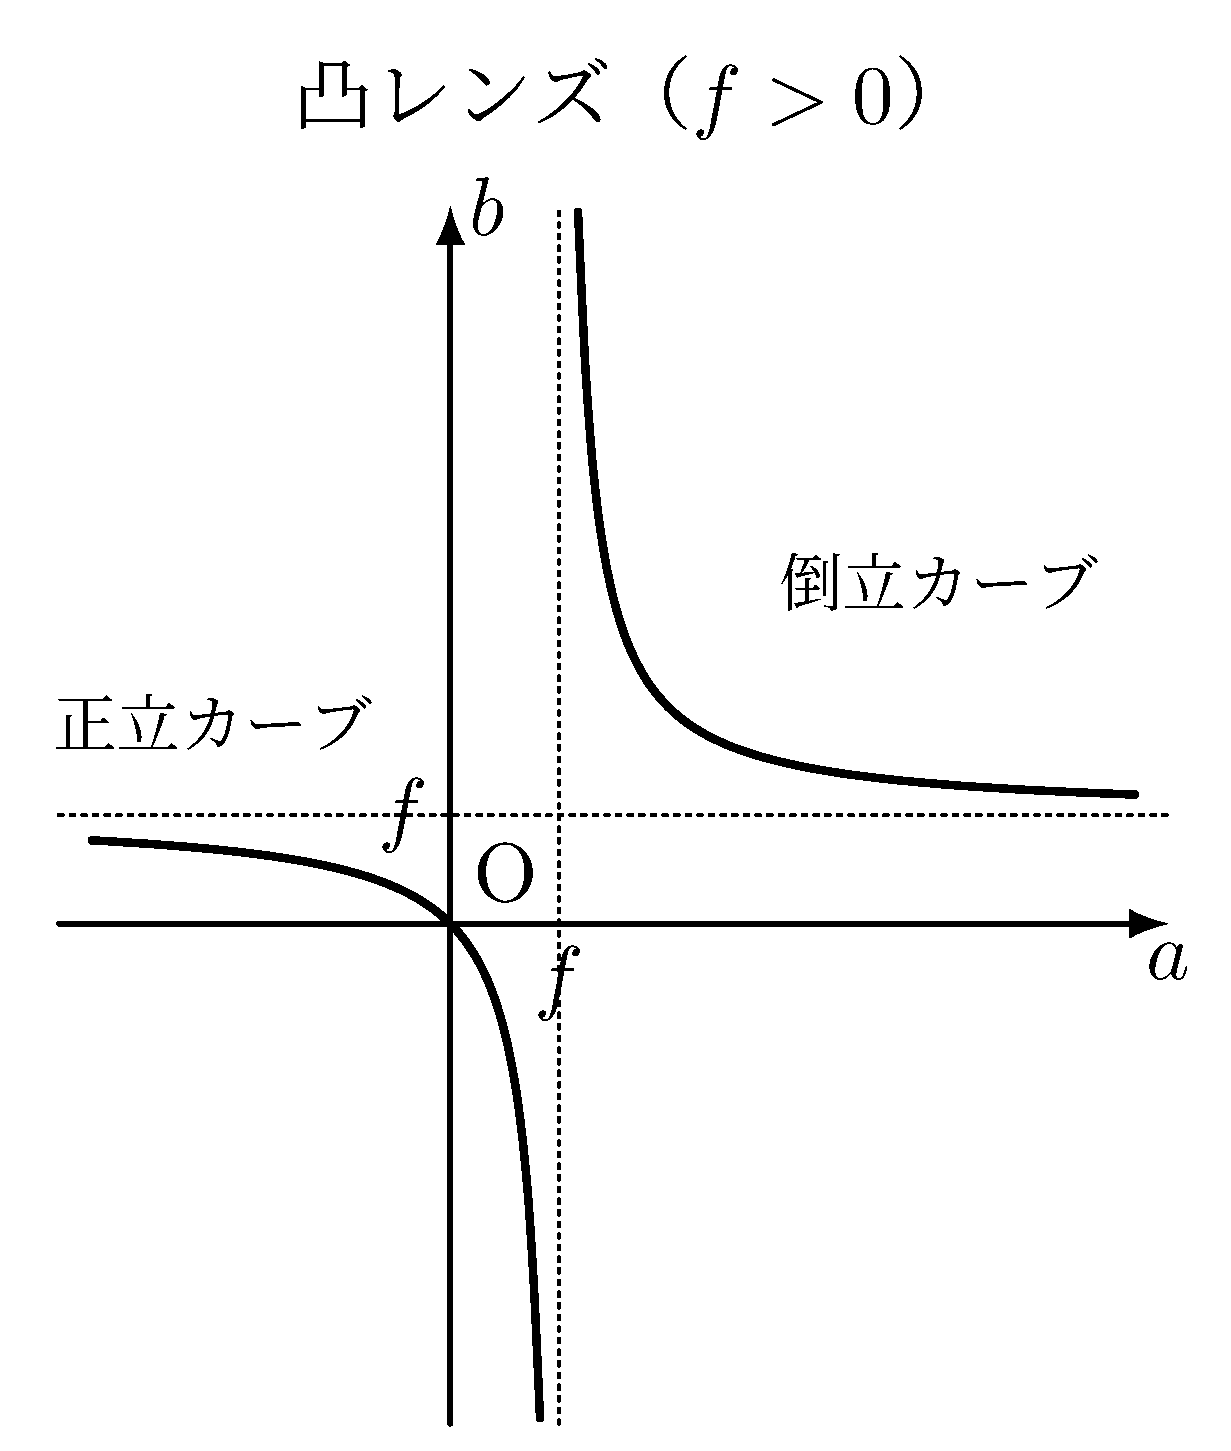
\includegraphics[keepaspectratio,width=66mm]{fig/n20_hyp_conv.png}\end{center}
       \[a>f\quad\text{もしくは}\quad a<0\]
       のいずれかの条件が満たされることが必要である．しかし，$a<0$とは虚光源を利用する場合であるから本問の場合にはそぐわない．よって，
       \[a>f\ (=12\U{cm})\]
       であることが条件である．

       以上より，スクリーンと光源との間の距離$a+b$に必要な条件を考えると，
       \[\begin{aligned}a+b&=\frac{a^2}{a-12}=\frac{1}{\dfrac{1}{a}-\dfrac{12}{a^2}}\\
         &=\frac{1}{\dfrac{1}{48}-12\left(\dfrac{1}{a}-\dfrac{1}{24}\right)^2}\\
         &=\frac{48}{1-\left(\dfrac{24}{a}-1\right)^2}\end{aligned}\]
       であり，$a$の変域は$a>12\U{cm}$であるから，$a+b$のとりうる範囲は，
       \[a+b\geqq 48\U{cm}\Ans\]
       （等号成立は$a=24\U{cm}$）
\end{komon}

\MonN{73}{虫めがね}\par\nopagebreak
\begin{sisin}
図から分かるように，虫めがねでは，{\gtfamily 目から見てレンズの向こう側}に物体（{\gtfamily 実光源}）を置き，{\gtfamily それと同じ側}に{\gtfamily 虚像}を作ってこれを見る．よって，写像公式を適用する場合には左側をレンズの手前側，右側をレンズの向こう側とみなし，$a>0$, $b<0$として公式に値を代入する必要がある．光源と像の種類をよく考えて，$a$, $b$の正負を考えれば，レンズのどちら側を手前側とみなして写像公式を利用すればよいのかが分かるはずである．
\end{sisin}
\KaiHead
\begin{komon}
\ko{1} 物体をレンズから距離$x\U{m}$だけ離して置くとする．
       \begin{center}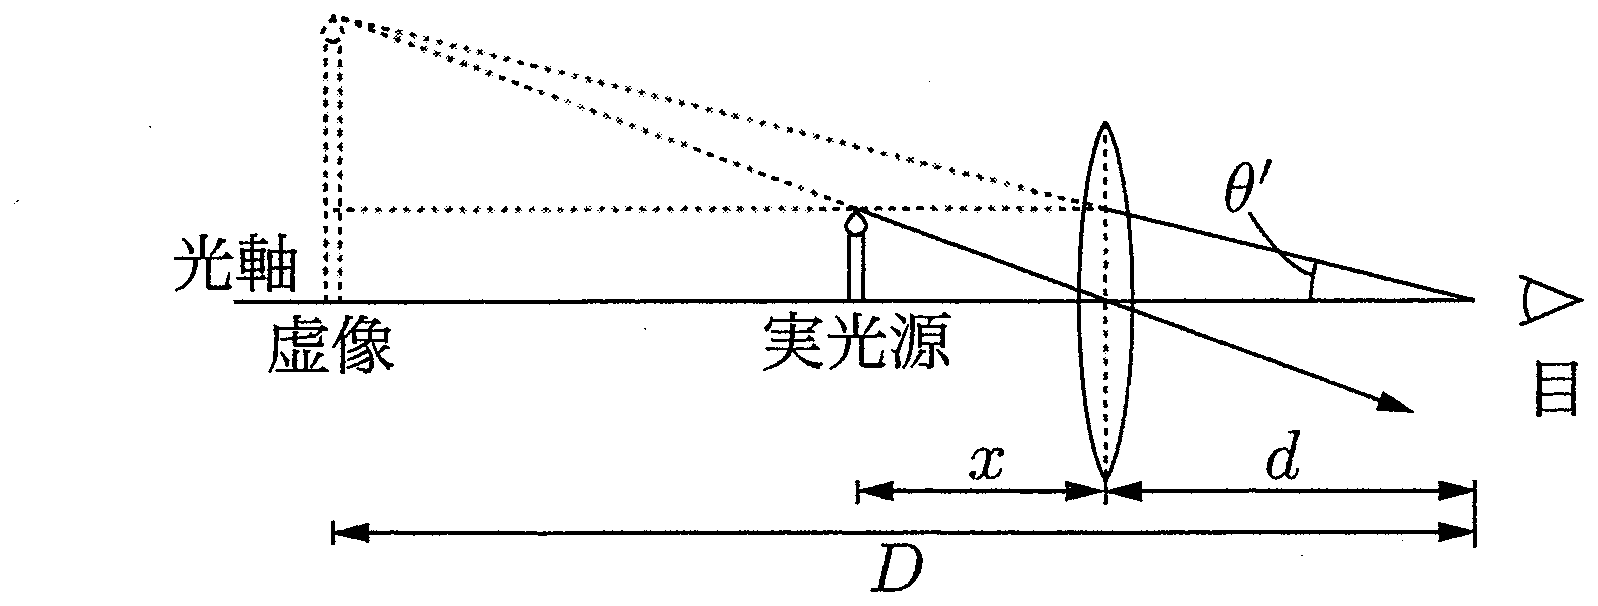
\includegraphics[keepaspectratio,width=62mm]{fig/n20_a73_zu1.png}\end{center}
       このとき，凸レンズに対して写像公式を適用すると，光源は実光源，像は虚像であるから$a>0$, $b<0$であり，$a=+x\U{m}$, $b=-(D-d)\U{m}$として代入すればよい．よって，
       \[\frac{1}{+x}+\frac{1}{-(D-d)}=\frac{1}{f}\]
       となる．これを解いて，
       \[x=\frac{f(D-d)}{f+D-d}\U{m}\Ans\]
\ko{2} 実光源の大きさを$y\U{m}$とすると，レンズなしで明視距離の位置にこの物体を置いたときの視角は，
       \begin{center}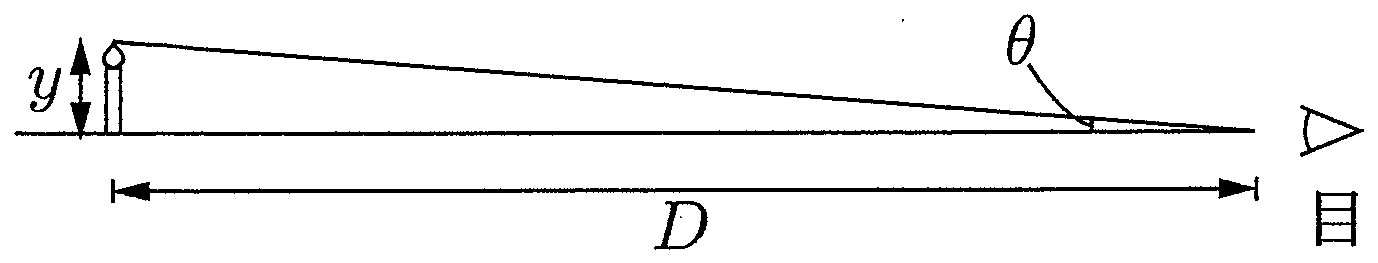
\includegraphics[keepaspectratio,width=62mm]{fig/n20_a73_zu2.png}\end{center}
       \[y=D\tan\theta\U{m}\]
       の関係を満たす．

       また，レンズを利用した場合には，
       \begin{center}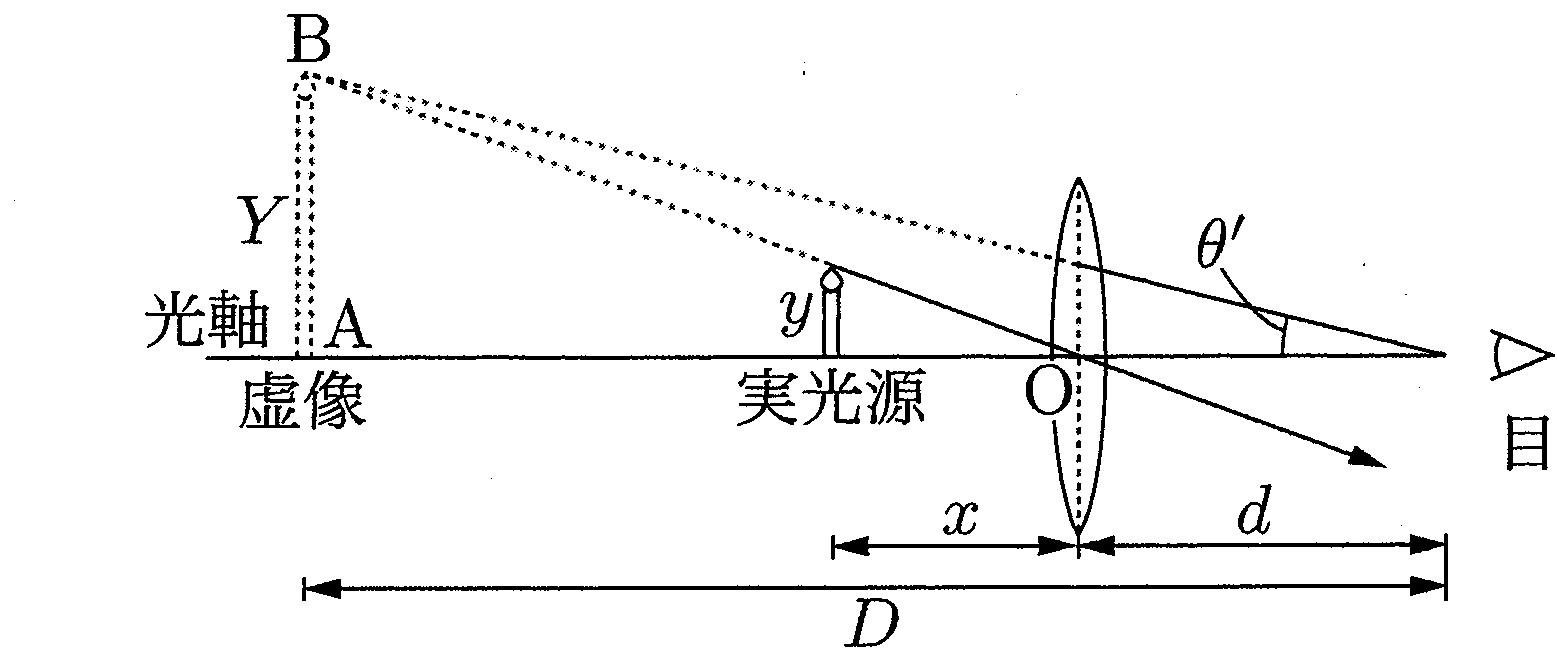
\includegraphics[keepaspectratio,width=62mm]{fig/n20_a73_zu3.png}\end{center}
       三角形$\mathrm{OAB}$の相似に着目すると，虚像の大きさは
       \[Y=\frac{D-d}{x}y\]
       であるから，レンズを通して明視距離の位置の虚像を見たときの視角は，目の位置を$\mathrm{C}$として三角形$\mathrm{ABC}$に着目することにより，
       \[Y=D\tan\theta^\prime\]
       である．

       $\theta$, $\theta^\prime\ll 1$に対する一次近似$\tan\theta\fallingdotseq\theta$, $\tan\theta^\prime\fallingdotseq\theta^\prime$を利用して倍率を求めると，
       \[\begin{aligned}M&=\frac{\theta^\prime}{\theta}\fallingdotseq\frac{\tan\theta^\prime}{\tan\theta}=\frac{Y/D}{y/D}\\
         &=\frac{D-d}{x}=1+\frac{D-d}{f}\Ans\end{aligned}\]
\end{komon}

\MonN[\Sitei]{74}{複合レンズ}\par\nopagebreak
\begin{sisin}
$\mathrm{A}$, $\mathrm{B}$の位置はすでに確定しているので，$\mathrm{A}$から出た光が最初に$\mathrm{B}$を通った後の光の進み方はすでに決まっており，問題となっているのは凹レンズ$\mathrm{C}$をどの位置におけばよいか，である．反射鏡$\mathrm{D}$で反射して光が左へ戻っていく際に，レンズ$\mathrm{B}$を通過して再び$\mathrm{A}$点に収束するためには，{\gtfamily 往路と復路が同じになっている}ことが必要であるから，そのことを利用して考えれば比較的簡単に解けるはずである．
\end{sisin}
\KaiHead
\hspace{1zw}点光源$\mathrm{A}$から出た光が$\mathrm{B}$を通過したときに出来る像の位置を求めると，$\mathrm{AB}$間の距離は$40\U{cm}$であるから，写像公式を利用して，
\[\frac{1}{40}+\frac{1}{b}=\frac{1}{20}\]
ゆえ$b=40\U{cm}$，すなわち$\mathrm{B}$を通過したのちにレンズの先$40\U{cm}$の位置に収束するように光は進む．
\begin{center}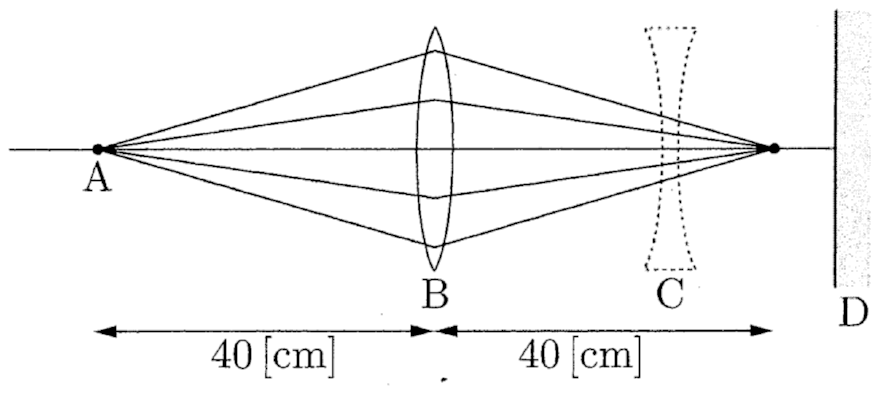
\includegraphics[keepaspectratio,width=62mm]{fig/n20_a74_zu1.png}\end{center}
\hspace{1zw}また，レンズに入射して屈折する光の経路は逆向きに光が進む場合でも全く同一になるので，反射鏡$\mathrm{D}$で反射したのち再び$\mathrm{A}$点で像を結ぶためには，上図に示したような経路でレンズ$\mathrm{B}$に再び入らなければならない．

\hspace{1zw}このことから，レンズ$\mathrm{C}$を置くときには，レンズ$\mathrm{C}$を通過した光が反射鏡$\mathrm{D}$によって反射される際に，再び全く同一の経路をたどってレンズ$\mathrm{C}$に戻らなければならず，それが満たされるのは次の2パターンに限定されるのは明らかである．

\hspace{1zw}\MARU{1}\ レンズ$\mathrm{C}$によって光が平行光となり，$\mathrm{D}$で垂直反射して再びレンズ$\mathrm{C}$に戻るパターン
\begin{center}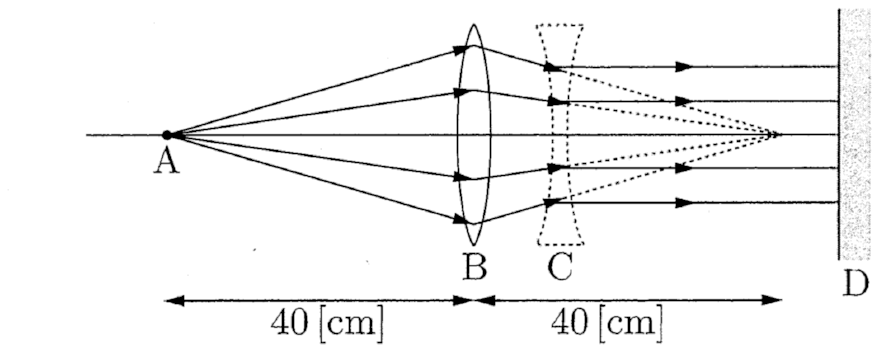
\includegraphics[keepaspectratio,width=62mm]{fig/n20_a74_zu2.png}\end{center}
\hspace{1zw}\MARU{2}\ レンズ$\mathrm{C}$によって光が収束していき，ちょうど鏡$\mathrm{D}$上に像を結んで一点に収束し，$\mathrm{D}$で反射して再びレンズ$\mathrm{C}$に戻るパターン
\begin{center}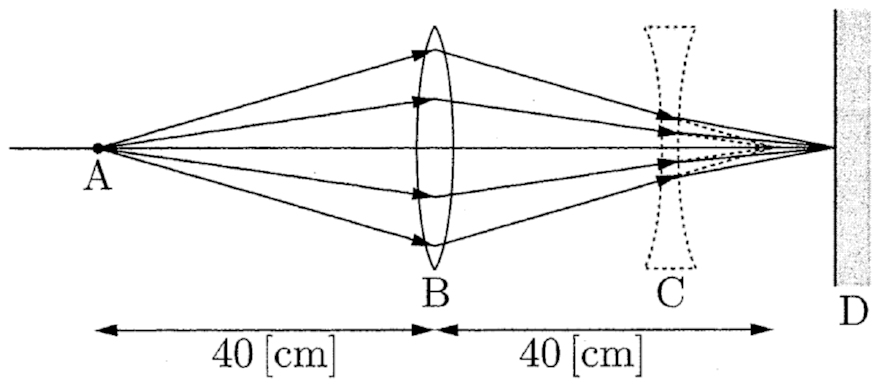
\includegraphics[keepaspectratio,width=62mm]{fig/n20_a74_zu3.png}\end{center}
\hspace{1zw}上述した2パターンの場合には$\mathrm{D}$によって反射した光は明らかに元の経路をたどってレンズ$\mathrm{C}$, $\mathrm{B}$を通過し再び$\mathrm{A}$に戻って像を結ぶことになる．これら以外の場合だと，反射鏡$\mathrm{D}$で反射した光は往路の経路をたどって戻らないため，再び$\mathrm{A}$に収束することはない．よって上述の二つの場合についての$\mathrm{DC}$間の距離を求めればよい．

\noindent{\gtfamily \MARU{1}の場合}

\hspace{1zw}これは明らかで，$\mathrm{B}$から右に$40\U{cm}$の地点（凸レンズ$\mathrm{B}$による光の収束点）が凹レンズ$\mathrm{C}$の焦点になっていればよい．
\begin{center}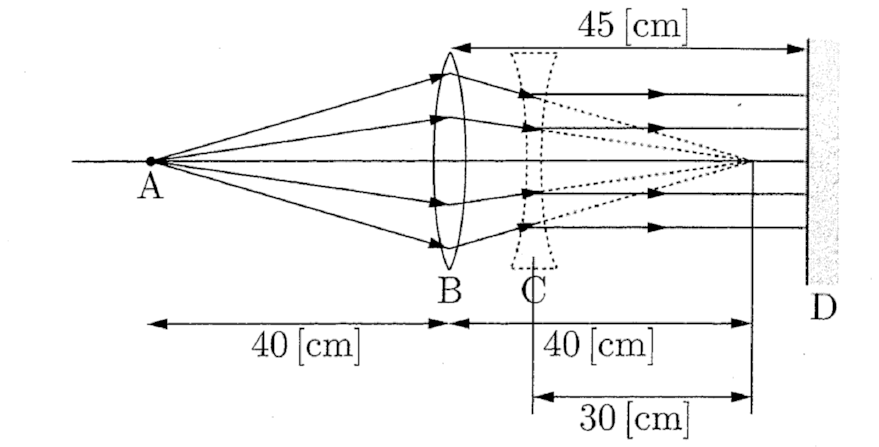
\includegraphics[keepaspectratio,width=62mm]{fig/n20_a74_zu4.png}\end{center}
\hspace{1zw}よって前図の位置関係から，このときの$\mathrm{DC}$間の距離は$35\U{cm}$であることが分かる．

\noindent{\gtfamily \MARU{2}の場合}

\hspace{1zw}このとき，凹レンズ$\mathrm{C}$を置く位置が$\overline{\mathrm{DC}}=x\U{cm}$であるとすると，凹レンズ$\mathrm{C}$に対しては凸レンズ$\mathrm{B}$によって$x-5\U{cm}$の位置に虚光源が存在する光の入射をすることが分かる．
\begin{center}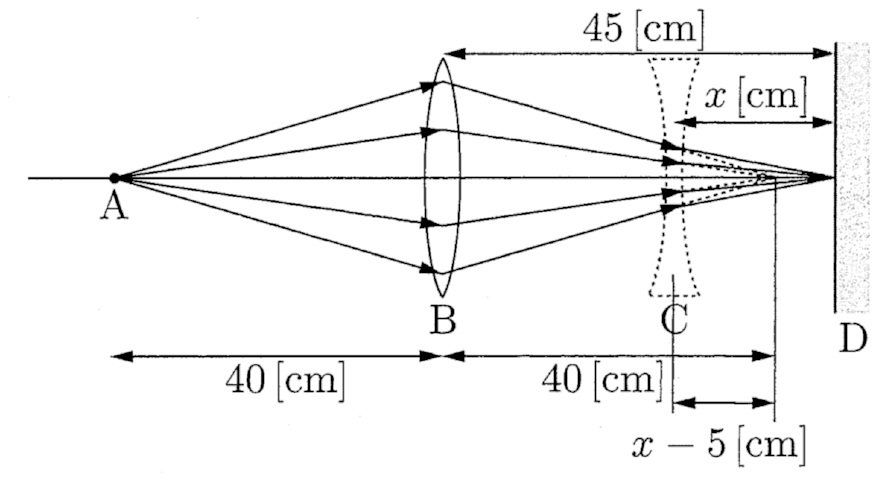
\includegraphics[keepaspectratio,width=62mm]{fig/n20_a74_zu5.png}\end{center}
\hspace{1zw}そして凹レンズ$\mathrm{C}$を通過したのち$\mathrm{D}$点に実像を結べばよいので，$\mathrm{C}$に対する写像公式は
\[\frac{1}{-(x-5)}+\frac{1}{x}=-\frac{1}{30}\]
となる．よってこれを整理して，
\[x^2-5x-150=0\]
を解いて，
\[x=+15\U{cm},\ -10\U{cm}\]
$x<0$は不適であるから，$\mathrm{DC}$間の距離を$15\U{cm}$にすればよいことが分かる．

\hspace{1zw}以上より，$\mathrm{DC}$間の距離を，$35\U{cm}$または$15\U{cm}$にすれば再び$\mathrm{A}$点で像を結ぶ．\hspace{0.25zw}\mbox{$\cdots$(答)}

\Rank{C問題}
\MonN{75}{顕微鏡}\par\nopagebreak
% 原本の（指針）は「B問題[73]と同様」だが，[73]は虫めがね（単レンズ）で複合レンズでは
% ない。複合レンズの前問［74］の誤りと判断して直した（2026-09-10）。
\begin{sisin}
複合レンズに関する問題は，B問題［74］と同様，{\gtfamily まず一つ目のレンズによる像を求め，次にそれを光源とみなしてもう一つのレンズによる像を求める}，という手順で考えよ．ひとつずつ順番に考えれば，複雑な問題といえどしょせんは単に一つ一つのレンズに対して写像公式を適用するだけの問題だと分かるはずである．
\end{sisin}
\KaiHead
\begin{komon}
\ko{1} $\mathrm{L_1}$から実像$\mathrm{BB^\prime}$までの距離を$b\U{cm}$とおき，凸レンズ$\mathrm{L_1}$に対して写像公式を適用すると，
       \[\frac{1}{a}+\frac{1}{b}=\frac{1}{f_1}\]
       であるから，これを解いて
       \[b=\frac{a}{a-f_1}f_1\U{cm}\Ans\hspace{2mm}\cdots\MARU{1}\]
\ko{2} 二つのレンズの焦点間の距離が$d\U{cm}$であるとき，$\mathrm{BB^\prime}$がレンズ$\mathrm{L_2}$に対してどれだけ下方向にあるのかを考えると，\par
       \begin{center}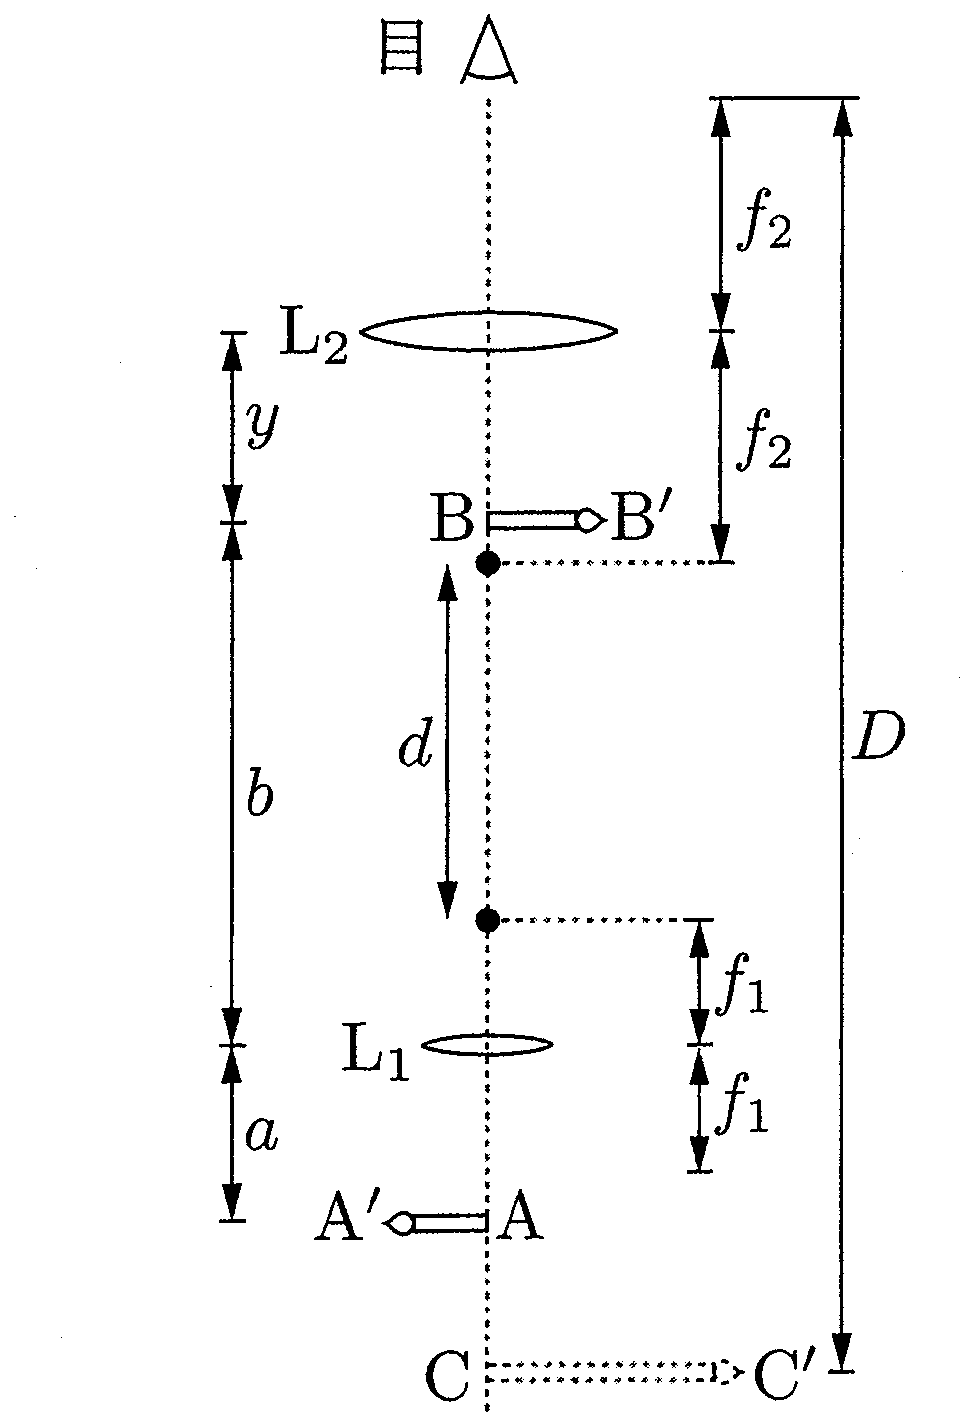
\includegraphics[keepaspectratio,width=46mm]{fig/n20_a75_zu1.png}\end{center}
       \[y=(f_2+d+f_1)-b=f_2+d-\frac{f_1^2}{a-f_1}\]
       だけ下方にある（この値が負であるのなら，$\mathrm{BB^\prime}$はレンズ$\mathrm{L_2}$の上方にある）．

       ここで，凸レンズの写像公式$(a-f)(b-f)=f^2$の直角双曲線を用いて考えると，凸レンズによって虚像が作られるためには，光源がレンズの手前側（すなわち虚像の作られている側，本問の場合だと$\mathrm{L_2}$の下側）にあり，なおかつそれが凸レンズの焦点の内側に入っていればよいことが分かる（次図参照）．
       \begin{center}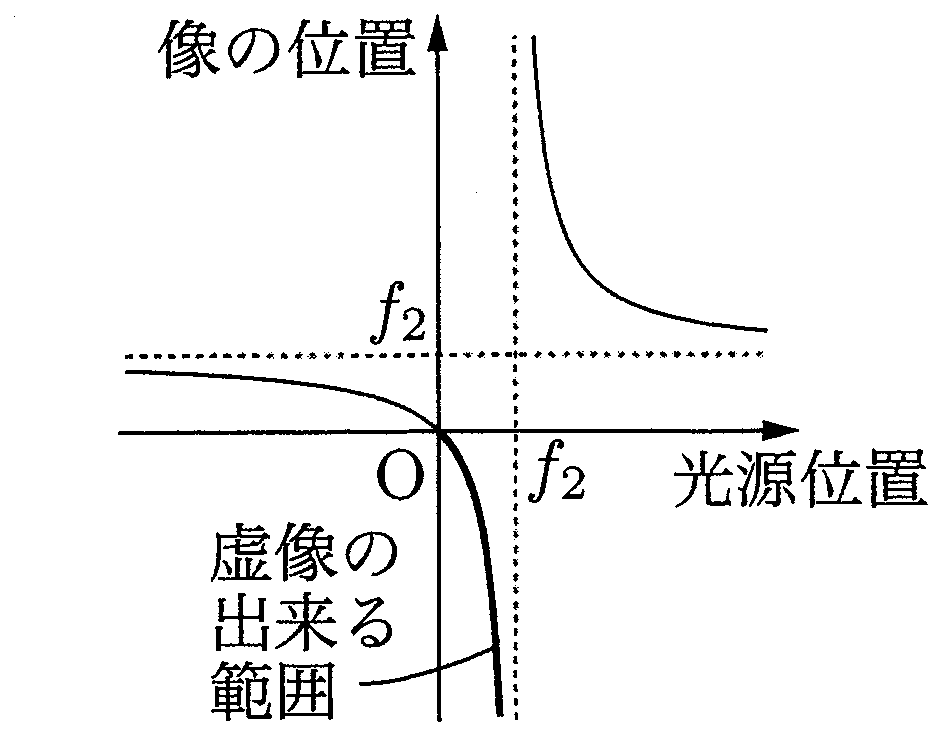
\includegraphics[keepaspectratio,width=54mm]{fig/n20_a75_zu2.png}\end{center}
       よって，レンズ$\mathrm{L_2}$によって虚像が出来るための条件は，
       \[0<f_2+d-\frac{f_1}{a-f_1}f_1<f_2\]
       である．これを解いて，
       \[\frac{f_1^2}{a-f_1}-f_2<d<\frac{f_1^2}{a-f_1}\Ans\]
\ko{3} (2)の条件が満たされる場合には虚像が出来るが，虚像が明視距離の位置に出来るためには，レンズ$\mathrm{L_2}$に対する写像公式より
       \[\frac{1}{+y}+\frac{1}{-(D-f_2)}=\frac{1}{f_2}\hspace{2mm}\cdots\MARU{2}\]
       が成立しなければならない．

       ここで，顕微鏡の倍率を考えると，まずレンズ$\mathrm{L_1}$によって元の物体が
       \[\mathrm{BB^\prime}=\left|\frac{b}{a}\right|\times\mathrm{AA^\prime}\]
       となり，これがレンズ$\mathrm{L_2}$によって，
       \[\mathrm{CC^\prime}=\left|\frac{D-f_2}{y}\right|\times\mathrm{BB^\prime}\]
       になるのだから，顕微鏡の倍率は，
       \[\left|\frac{\mathrm{CC^\prime}}{\mathrm{AA^\prime}}\right|=\frac{D-f_2}{y}\cdot\frac{b}{a}\]
       となる．まず\MARU{2}より，
       \[\frac{1}{y}=\frac{1}{D-f_2}+\frac{1}{f_2}\]
       であるから，
       \[\begin{aligned}\frac{D-f_2}{y}\cdot\frac{b}{a}&=\left(1+\frac{D-f_2}{f_2}\right)\cdot\frac{b}{a}\\
         &=\frac{D}{f_2}\cdot\frac{b}{a}\end{aligned}\]
       である．さらに\MARU{1}を利用すると，顕微鏡の倍率は
       \[\left|\frac{\mathrm{CC^\prime}}{\mathrm{AA^\prime}}\right|=\frac{D}{f_2}\cdot\frac{f_1}{a-f_1}\Ans\]
       \begin{bsHosoku}{参考}
       本問ではここまでの変形しか要求されていないが，実際には筒の長さ$d\U{cm}$が決まると明視位置に虚像を作るために$\mathrm{AA^\prime}$を置く位置$a\U{cm}$が決まるため，顕微鏡の倍率は$d$, $D$, $f_1$, $f_2$の四つで表すことができる．計算をすると，
       \[\left|\frac{\mathrm{CC^\prime}}{\mathrm{AA^\prime}}\right|=\frac{dD+f_2^2}{f_1f_2}\]
       となり，これが一般的な顕微鏡の倍率である．
       \end{bsHosoku}
\end{komon}

\end{multicols}
